% !TEX program = lualatex
% 認知の肥満 — Option A: Theory-First Structure
% LuaLaTeX + luatexja で日本語組版
\documentclass[a4paper,11pt,titlepage]{article}

%%% ===== パッケージ =====
\usepackage{luatexja}
\usepackage{luatexja-fontspec}
\usepackage[hiragino-pron]{luatexja-preset}   % macOS Hiragino 自動設定
\usepackage[margin=25mm]{geometry}
\usepackage{amsmath,amssymb}
\usepackage{booktabs}
\usepackage{longtable}
\usepackage{graphicx}
\usepackage{hyperref}
\usepackage{cleveref}
\usepackage{enumitem}
\usepackage{xcolor}
\usepackage{float}
\usepackage{caption}
\usepackage{setspace}
\usepackage[numbers,sort&compress]{natbib}

%%% ===== ハイパーリンク設定 =====
\hypersetup{
  colorlinks=true,
  linkcolor=blue!60!black,
  citecolor=green!50!black,
  urlcolor=blue!70!black,
  bookmarksnumbered=true,
}

%%% ===== 行間 =====
\setstretch{1.25}

%%% ===== カスタムコマンド =====
\newcommand{\balanceL}{L}
\newcommand{\cogInput}{I}
\newcommand{\expProc}{C}

%%% ===== タイトル =====
\title{%
  \vspace{-2cm}
  {\LARGE\bfseries 認知の肥満}\\[6pt]
  {\large 認知体験不均衡による鬱・暴力・情報過負荷の統合的枠組み}\\[12pt]
  {\normalsize\itshape Cognitive Obesity: Cognitive-Experiential Imbalance\\
   as a Unifying Framework for Depression, Violence, and Information Overload}\\[12pt]
  {\small 探索的研究論文 \quad 草稿: 2026年3月}\\
  {\small\color{red} ステータス: 探索的研究 --- 確認的検証は未完}
}
\author{独立研究者}
\date{}

% ================================================================
\begin{document}
\maketitle
\thispagestyle{empty}

% ================================================================
% Abstract
% ================================================================
\begin{abstract}
\noindent
本論文は、デジタルメディアとメンタルヘルスの関係をめぐる論争に対し、栄養代謝アナロジーに基づく統合的枠組を提案する。
中核的主張は、精神病理の主要な予測因子はスクリーンタイムの絶対量ではなく、非選択的認知入力と体験的処理のバランス（加法的不均衡）であり、その質的分類基準は感覚運動ループ閉合度---環境との双方向的因果結合の有無---である、というものである。

177ヶ国$\times$1990--2023年パネルデータの系統的分析（Study~1）により、以下を示す:
(1)~Country~FEのみで観察されたインターネット普及率の正の効果は、Two-Way Fixed Effects（TWFE）で符号が反転し、共通時間トレンドに依存していた。
(2)~鬱病有病率の最強の予測因子はGDP（$t=18.27$）であり、診断バイアスが支配的であることが、ハードアウトカム（自殺率）との比較で確認された。
(3)~Hansen PTRにより自殺率では閾値$\gamma^*=25.7$（$F=213$、保護効果の飽和）が同定される一方、鬱病では不連続な閾値は検出されず（$p=0.654$）、連続的な逆U字型dose-response（二次項$F=127.0$）が最適フィットとなる。
(4)~広告曝露プロキシ（Internet$\times$GDP/capita）はこの恩恵--害反転をより明瞭に捕え（閾値$\approx$\$1,000）、1階差分分析でGDP変化を統制した後も有意に鬱病を予測した（$t=3.16$、internet $>30\%$サブサンプル）。

個人レベルの検証（NHANES $N=5{,}032$; ATUS $N=21{,}736$）では、身体運動と能動的認知余暇が独立の加法チャネルとして幸福度を予測し（交互作用$p=0.95$）、両方の不在が最悪の健康転帰を生むことが確認された（Fair/Poor健康率3.1倍）。
行動経済学・環境心理学・神経科学の既存知見をバランスモデルで再解釈し、個人レベルの収束的証拠を提示する。

重大な限界として、マクロレベルの知見は全て生態学的誤謬の制約を受ける---国レベルの関連を個人レベルのメカニズムに直接帰属することはできない。
本研究は探索的であり、経験サンプリング法（ESM）による個人レベルの確認的検証を必要とする。反証条件を明示する。
\end{abstract}

\newpage
\tableofcontents
\newpage

% ================================================================
% Section 1: Introduction
% ================================================================
\section{導入}\label{sec:introduction}

2020年代、先進国のメンタルヘルス統計は奇妙な逆説を示している。物質的には歴史上最も恵まれた世代が、歴史上最も高い鬱病有病率を記録している。暴力犯罪が減り続ける社会で、若者の自傷と希死念慮が増え続けている。人々はかつてないほど多くの「つながり」を持ちながら、かつてないほど孤独を報告している。

\subsection{パラドックスの提示}

この逆説をめぐり、2つの陣営が対立している。一方の規制派（Haidt, 2024; Twenge, 2017; Hansen, 2019）はスマートフォンとSNSへの曝露制限を主張する。青少年の精神疾患の急増はスマートフォン普及と並行しており、Hansenの『スマホ脳』（2019）の世界的ベストセラー化はこの懸念が広範な社会的共鳴を得ていることを示す。他方のデジタルレジリエンス派は、効果量が極めて小さい---眼鏡の着用やジャガイモの摂取と同程度---と反論し（Orben \& Przybylski, 2019）、縦断研究では持続的な害は示されないとし（Heffer et al., 2019; Coyne et al., 2020）、メディアリテラシー教育を処方する。一般精神病理因子（$p$因子; Caspi et al., 2014）の研究は、内在化・外在化症状が共通の負荷次元を共有することを示唆しており、本フレームワークはこの共有分散を生成するメカニズムとして処理容量の過負荷を提案することで、この知見を拡張する。Facebook非活性化のRCTはウェルビーイングの改善を示したが、同時に政治的知識とニュース認知の減少を伴い（Allcott et al., 2020）、単純な制限も単純な教育もこの複雑性を解決できないことを示している。

しかし約10年にわたる論争は収束の兆しを見せない。なぜか。

\subsection{既存論争の構造的問題}

本論文の主張は、\textbf{両陣営とも見ている変数が間違っている}、というものである。議論はスクリーンタイムの絶対量に焦点を当てているが、真に重要なのは認知入力と体験的処理のバランスである。

これは栄養学と構造的に同型である。肥満の原因は「食べること」そのものではなく、カロリー摂取と代謝消費の不均衡である。規制派は「カロリーを減らせ」と言い、リテラシー派は「栄養素の質を上げれば量は問題ない」と言う。しかしどちらも、患者が運動していないという本質的な問題を見落としている。

ここで「認知入力」と呼ぶものの本質は、単なる情報量ではない。SNSのフィードは、私たちを毎日数百人の他者の内的状態に曝す。それぞれの投稿が暗黙的に自己との比較を要求する。嫉妬、不全感、共感疲れ---認知的に最もコストの高い感情群が、休む間もなく喚起される。かつて感情には、それを感じ、身体で味わい、消化する時間があった。雨の匂いを嗅ぎ、散歩し、友人と顔を突き合わせて語る中で、経験は処理された。現代の情報環境は、この消化の時間を構造的に奪っている。

さらに根本的な問題がある。デジタルプラットフォームのアルゴリズムは「エンゲージメント」を最適化する。人間の感情は、この最適化関数の入力変数として離散化される。連続的で曖昧で文脈依存だった感情体験が、6択のリアクションボタンに圧縮される。そして人間の側が---機械より圧倒的に柔軟であるがゆえに---その離散カテゴリに収まるように感情の表出を調整し始める。「バズる怒り方」が存在するという事実が、この構造的非対称性を端的に示している。

\subsection{本論文の主張と貢献}

本論文はこの問題構造を「認知の肥満（Cognitive Obesity）」と名付ける。身体の肥満がカロリー摂取と消費の加法的バランス不均衡（$EB = \text{Intake} - \text{Expenditure}$）から生じるように、認知の肥満は認知入力と体験的処理のバランス不均衡から生じる。

この枠組みは
(a)~なぜスクリーンタイム論争が収束しないかを説明し（両陣営ともバランスの入力側のみを見ている）、
(b)~177ヶ国のパネルデータから検証可能な予測を生成し、
(c)~鬱病・暴力・情報過負荷を処理容量超過の異なる発現形として統一的に扱う。

本論文の構成は以下の通りである。\cref{sec:theory}で理論枠組みを構築し、バランスモデルの数理的定式化と検証可能な予測を導出する。\cref{sec:macro}でこれらの予測を177ヶ国$\times$34年のマクロパネルデータで検証する。\cref{sec:individual}で個人レベルの証拠（直接分析および既存知見の再解釈）を提示する。\cref{sec:operationalization}で操作化と確認的検証デザインを提案し、\cref{sec:falsification}で反証条件を明示する。


% ================================================================
% Section 2: Theoretical Framework
% ================================================================
\section{理論枠組み}\label{sec:theory}

\subsection{栄養代謝アナロジーとバランスモデル}\label{sec:analogy}

提案する枠組みは、栄養代謝と認知処理の間に構造的アナロジーを描く（\cref{tab:analogy}）。

\begin{table}[htbp]
\centering
\caption{栄養代謝---認知処理のアナロジー}
\label{tab:analogy}
\begin{tabular}{lll}
\toprule
 & 栄養学 & 認知 \\
\midrule
入力 & カロリー摂取 & 情報入力（スクリーン時間、メディア、記号的コンテンツ） \\
処理 & 代謝消費 & 体験的処理（身体活動、感覚運動的関与） \\
圧縮 & 栄養素の吸収・貯蔵 & 教育・内省・睡眠による抽象化 \\
病理 & 肥満（摂取$\gg$消費） & 「感情の肥満」（認知入力$\gg$体験的処理） \\
閾値 & メタボリックシンドローム & 鬱病、不安、処理破綻 \\
\bottomrule
\end{tabular}
\end{table}

このアナロジーは単なる比喩ではない。具体的な検証可能な予測を生成し（\cref{sec:operationalization}）、なぜスクリーンタイム論争が収束しないかを説明する。両陣営とも絶対量を測定しているが、病理はバランス依存である。ここで「バランス」とは加法的不均衡（$\balanceL = \alpha_1 \cdot \text{入力} - \alpha_2 \cdot \text{処理}$）を指す。栄養学のエネルギーバランス方程式（$EB = \text{Intake} - \text{Expenditure}$）が比率ではなく差分であるのと同様に、認知領域でも入力と処理は独立の加法チャネルとして病理に寄与する（\cref{sec:individual}で実証）。

先行研究について: Whitworth~(2009)が情報過負荷に対する同様の栄養メタファーを提案しているが、疫学データや操作化がない。近年、Foley~(2025)が``Cognitive Obesity''という表現をAI時代に用いたが比喩的指摘にとどまる。本枠組みは(a)~国際的統計的証拠の提供、(b)~処理モード理論への接地、(c)~反証可能な予測の導出の点でこれらの先行と異なる。

本枠組みが定式化する処理モードの区別には、いくつかの理論的伝統が収束している。Csikszentmihalyiの「フロー」概念（1990）は、感覚運動フィードバックループが密に閉じた状態---行為と意識が融合し自己参照的認知が停止する状態---を記述する。Nolen-Hoeksemaの反芻理論（1991）はその病理的対極を同定する: 行動的閉合を持たない反復的・自己集中的認知ループである。自己決定理論（Ryan \& Deci, 2000）は、有能感と自律性---いずれも閉じた行為-結果ループを必要とする---を基本的心理欲求として同定する。身体化された認知の伝統（Varela, Thompson, \& Rosch, 1991）は、認知が脱身体化された情報処理ではなく環境との感覚運動的結合によって根本的に構成されると論じる。Kaplanの注意回復理論（1995）は、自然環境が不随意的（ボトムアップ、感覚運動的）注意を関与させつつ随意的（トップダウン、認知的）処理を休ませることで注意を回復すると主張する。本枠組みはこれらの観察を単一の定量モデルに統合する: これらの理論が独立に適応的と記述する状態はいずれも高い感覚運動ループ閉合度（第2項）で特徴づけられ、病理的と同定する状態は低いループ閉合度と高い認知入力（第1項）を共有する。

\begin{figure}[htbp]
\centering
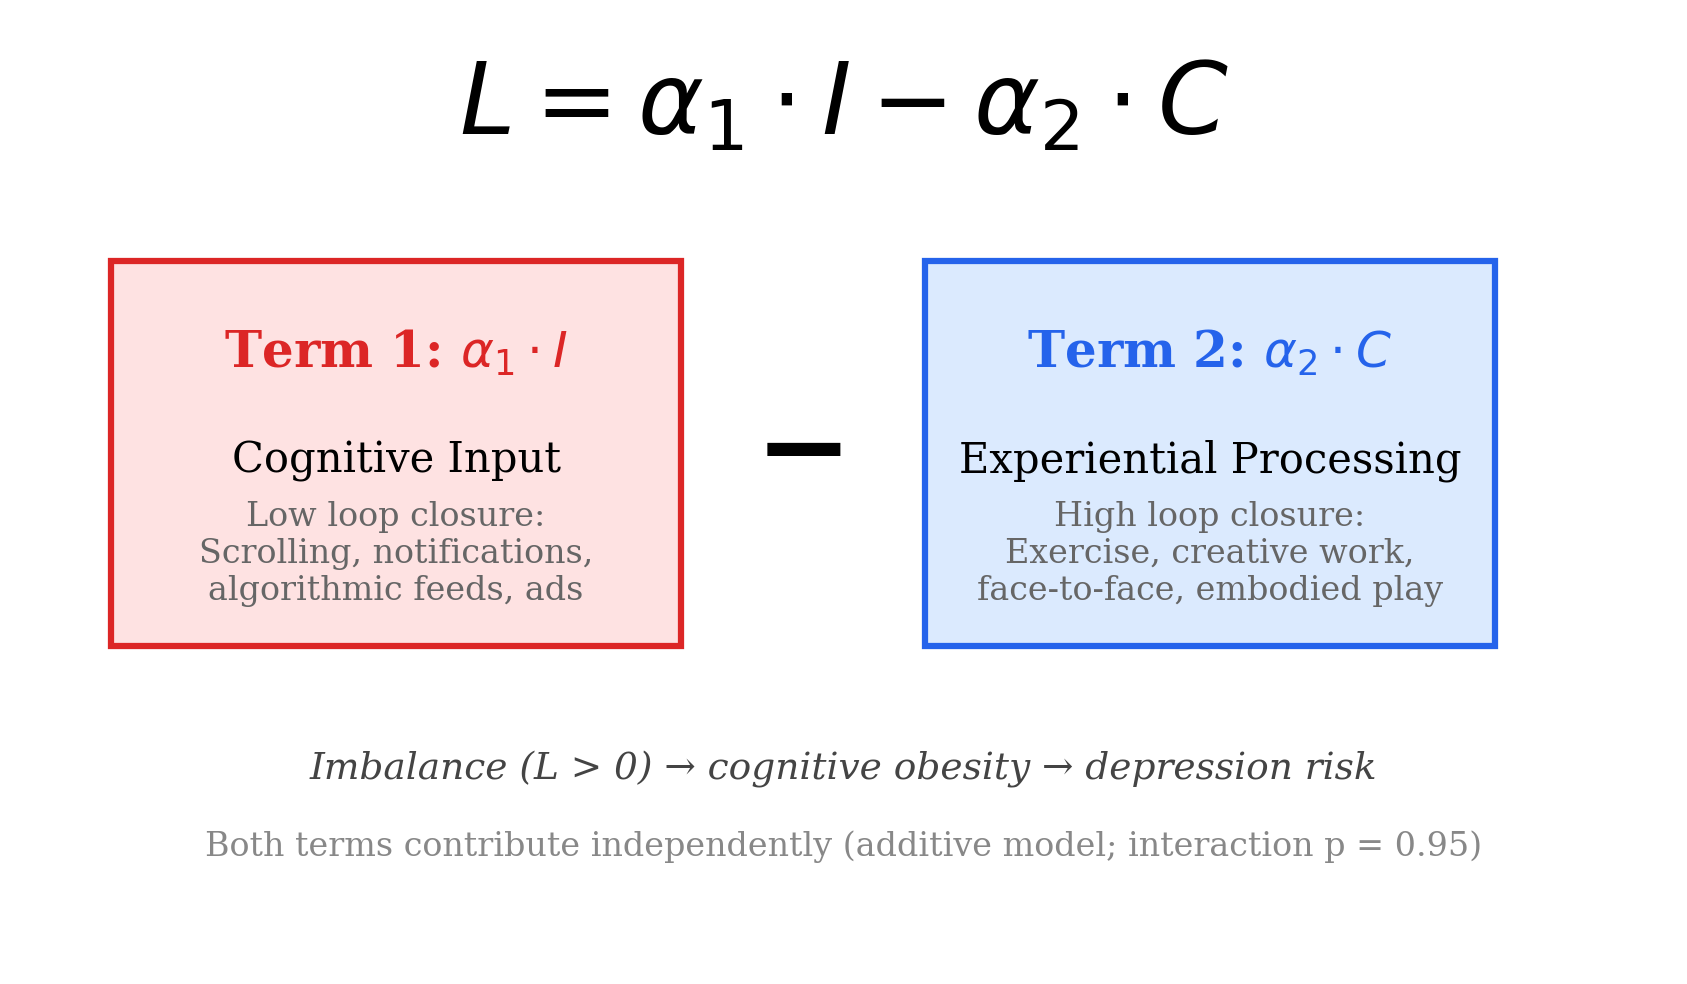
\includegraphics[width=0.85\textwidth]{fig01_balance_model.png}
\caption{認知負荷のバランスモデル: $L = \alpha_1 \cdot I - \alpha_2 \cdot C$。Term~1（認知入力）とTerm~2（体験的処理）は独立の加法チャネルとして寄与する（交互作用 $p = 0.95$）。}
\label{fig:balance-model}
\end{figure}


\subsection{認知負荷の非対称蓄積メカニズム}\label{sec:mechanism}

前節のアナロジーは問題の構造を記述する。本節ではそのメカニズムに踏み込む: なぜ先進国において特にバランスが病理的になるのか。

\subsubsection{感情粒度と処理コスト}

Barrettの構成主義感情理論によれば、感情カテゴリーは文化的に構成され、発達とともに分化する。「怒り」は「憤慨」「苛立ち」「義憤」「嫉妬」などに分化する。この分化は適応的である: 高い粒度はより文脈に適切な反応を可能にする。

しかし粒度には維持コストがある。$n$個の感情カテゴリーがあると、潜在的な関係構造は$O(n^2)$となる。先進国の住民は絶えず細かい感情弁別を行っている。この弁別自体が認知資源を消費する。非対称性の本質は、低所得国が感情カテゴリーが少ないのではなく、その社会環境が単位時間当たりの弁別イベント数を少なくすることにある。

\subsubsection{情報入力は一方的に処理コストを増大させる}

SNSとデジタルメディアは、2つのメカニズムでこの非対称性を増幅する:

\begin{description}[leftmargin=2em]
\item[(a) 曝露量] 他者の内的状態に接触する日常的な頭数は、デジタルメディア以前は物理的に制約されていた（Dunbar数と地理的近接性）。SNSはこれを日に数百から数千に増大させる。各接触が感情弁別を要求する。
\item[(b) 自己参照的比較] 他者の投稿は暗黙的に自分の生活との比較を要求する。これは社会的感情---嫉妬、不全感、自己評価---を活性化する。認知的に最も処理コストの高い感情群である。
\end{description}

\subsubsection{教育は圧縮として機能する}

教育は抽象化を通じて処理コストを低減する。「この10個の感情反応はすべて『喪失反応』の事例である」と認識することで、10個の個別処理イベントを1つに圧縮できる。これが教育の回帰係数が負（鬱病低減）である理由を説明する。


\subsection{数理的定式化}\label{sec:math}

前節までの言語的モデルを、検証可能な数理的形式に変換する。時点$t$における個人（または国）$i$の認知入力を$\cogInput_{i,t}$、体験的処理容量を$\expProc_{i,t}$として、認知負荷$\balanceL_{i,t}$を以下で定義する:
\begin{equation}\label{eq:balance}
  \balanceL_{i,t} = \alpha_1 \cdot \cogInput_{i,t} - \alpha_2 \cdot \expProc_{i,t}
\end{equation}
ここで加法バランスモデルを用いる理論的根拠は三つある。第一に、栄養学の標準的エネルギーバランス方程式が加法的差分であり、本稿の認知代謝アナロジーはこの構造と整合する。第二に、個人レベルデータ（NHANES $N=5{,}032$; ATUS $N=21{,}736$）で認知入力と体験的処理の交互作用は非有意であり（\cref{sec:individual}）、両者は独立の加法チャネルとして精神病理に寄与する。第三に、加法モデルは「インターネット普及率が同一でも、運動量が異なれば鬱病リスクが異なる」という知見を自然に説明する。

鬱病リスク$D_{i,t}$は、認知負荷$\balanceL_{i,t}$のロジスティック関数として定式化する:
\begin{equation}\label{eq:logistic}
  D_{i,t} = \sigma(\balanceL_{i,t} - \theta)
  = \frac{1}{1 + \exp\bigl(-(\balanceL_{i,t} - \theta)\bigr)}
\end{equation}
ここで$\alpha_1, \alpha_2$は各チャネルの感受性パラメータ、$\theta$は閾値パラメータ（リスクが急上昇する認知負荷の臨界値）である。

\subsubsection{閾値モデルの統合}

以上を統合する:
\begin{itemize}
  \item 処理コスト $= f(\text{感情粒度} \times \text{情報入力量})$ --- 発展とともに連続的に増大
  \item 処理容量 $= g(\text{教育による圧縮、体験的処理、睡眠による回復})$ --- 意図的な投資が必要
  \item 鬱病 $=$ 処理コストが処理容量を慢性的に超過した状態
  \item 急性危機（自殺・暴力）$=$ 処理コストが急性閾値を超過
\end{itemize}
このモデルは相関構造が高所得国でのみ出現する理由を説明する。低所得国では処理コストがまだ処理容量を超えておらず、鬱病・自殺・殺人は独立の外的原因に支配されている。高所得国では外的原因が抑制され、処理容量が律速段階となる。

\subsubsection{マクロレベルへの適用}

国$j$の年$t$における集団レベルバランスを以下で近似する:
\begin{align}
  \bar{R}_{j,t} &\approx \frac{\text{Internet}_{j,t}}{\text{Education}_{j,t}}
  \quad\text{(第一近似)} \label{eq:proxy-first} \\
  \text{AdProxy}_{j,t} &= \text{Internet}_{j,t} \times \text{GDP/capita}_{j,t}
  \quad\text{(精緻化)} \label{eq:proxy-ad}
\end{align}
式\eqref{eq:proxy-first}は最も単純なマクロ代理変数であるが、TWFEで符号が反転し不十分であることが示された（\cref{sec:twfe-collapse}）。式\eqref{eq:proxy-ad}の広告曝露プロキシは、非選択的認知入力（ターゲティング広告、アルゴリズム推薦、プッシュ通知）の密度を近似し、1階差分分析でGDPから独立した予測力を持つことが確認された（\cref{sec:first-diff}）。

\paragraph{限界の明記.}
式\eqref{eq:balance}--\eqref{eq:logistic}は静的モデルであり、バランスの時間的変動パターン（慢性的な過負荷 vs 間欠的な過負荷）を区別しない。動的拡張は将来の課題とする。


\subsection{感覚運動ループ閉合度による質的分類}\label{sec:loop-closure}

すべてのスクリーンタイムが等価ではない。本枠組みは、メンタルヘルスへの影響が活動の\textbf{感覚運動ループ閉合度}に依存すると予測する。

\paragraph{閉じたループ（適応的）.}
認知入力が運動出力につながり、それが環境フィードバックを生成し、それが次の認知を更新する活動。例: ビデオゲーム（入力$\to$判断$\to$運動行為$\to$視覚フィードバック$\to$調整）、創作活動、科学的探究。

\paragraph{開いたループ（不適応的）.}
認知入力が感覚運動サイクルを完結しない活動。例: 受動的SNS消費（入力$\to$感情反応$\to$スクロール; スクロールはコンテンツと運動的に無関係）、受動的動画視聴。

\paragraph{自己参照ループ（最も病理的）.}
処理の出力が外的接地なくそれ自体の入力となる活動。例: 反芻（思考$\to$思考の分析$\to$分析の分析$\to$\ldots）、エコーチェンバー（信念$\to$確証情報探索$\to$信念強化$\to$\ldots）。

\subsubsection{処理モード理論との接続}

Watkins \& Teasdale~(2001, 2004)は自己焦点的処理の2つのモードを区別する: 抽象的分析的モード（評価的・脱文脈的・原因--意味--結果に焦点）と、具体的体験的モード（直接的・非判断的・現在の瞬間的気づき）。抽象的分析的モードは鬱病における不適応的帰結と一貫して関連し、具体的体験的モードは保護的効果を示す。

感覚運動ループ枠組みはこの区別に直接対応する: 閉じたループは具体的体験的処理を強制し（環境フィードバックが現在の瞬間への関与を要求）、開いたループと自己参照ループは抽象的分析的処理にデフォルトする。

\subsubsection{体験的処理の操作的定義}

以上のループ閉合度の区別から、加法的バランスモデル$\balanceL = \alpha_1 \cdot \cogInput - \alpha_2 \cdot \expProc$の2項の操作的定義を明示する。第1項$\alpha_1 \cdot \cogInput$は「認知入力」（入力チャネル）---ループ閉合度が低い情報処理---を、第2項$\alpha_2 \cdot \expProc$は「体験的処理」（処理チャネル）---ループ閉合度が高い身体的・感覚的処理---をそれぞれ表す。

重要な点として、この区別は「認知的 vs 身体的」ではない。分類基準はループ閉合度---すなわち行為者の出力が環境からのフィードバックを即時的に生成し、そのフィードバックが次の処理を更新するサイクルの完結度---である。

\subsubsection{ビデオゲーム: 分類原理の試金石}

ゲーム研究は近年、「ゲーム＝有害」という一枚岩の見方から「ゲームの種類と関与の質による」へとパラダイムシフトしている（Granic et al. 2014; Johannes et al. 2021）。本枠組みはこの知見を統一的に説明する。創造型ゲーム（Minecraft等）および対戦型ゲーム（将棋、competitive FPS等）は高いループ閉合度を持ち、第2項に分類される。一方、ガチャ周回・レベル上げグラインド・放置系ゲームはループ閉合度が低く第1項に近づく。より広く言えば、ギャンブルやガチャは\emph{擬似閉ループ}の典型例である: 行動$\to$結果の系列は真の閉ループに見えるが、結果がスキルではなく確率に依存するため学習の蓄積が生じない。この「真の閉合 vs 擬似閉合」の区別は、ギャンブル障害と問題的ゲーム使用を共通のループ構造から統一的に記述する可能性を持つ。

重要な限界として、同一ゲームであっても個人の関与モードによって閉合度は変動する。厳密な測定にはESMによる個人の主観的関与度のリアルタイム評価が必要であり（\cref{sec:operationalization}参照）、これは本枠組みの最も重要な操作化上の課題である。

\begin{figure}[htbp]
\centering
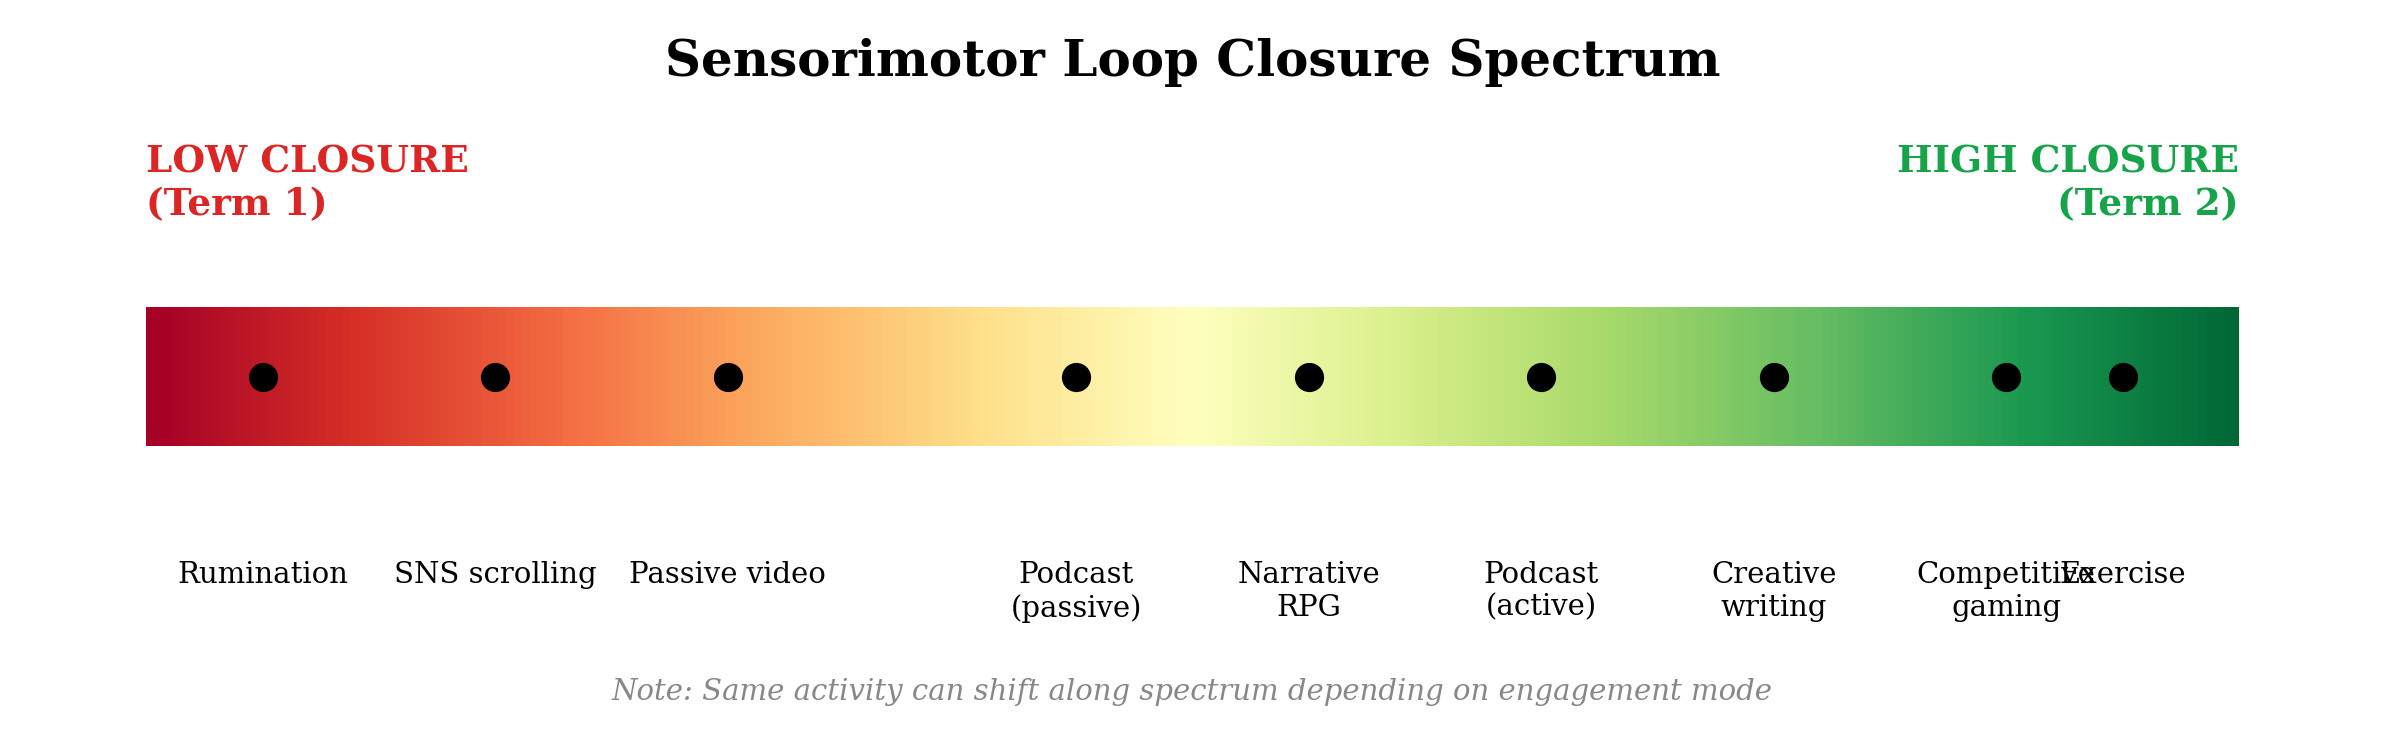
\includegraphics[width=\textwidth]{fig05_loop_closure_spectrum.png}
\caption{感覚運動ループ閉合度スペクトラム。同一活動でも関与モードによりスペクトラム上の位置は変動する。}
\label{fig:loop-spectrum}
\end{figure}

\begin{figure}[htbp]
\centering
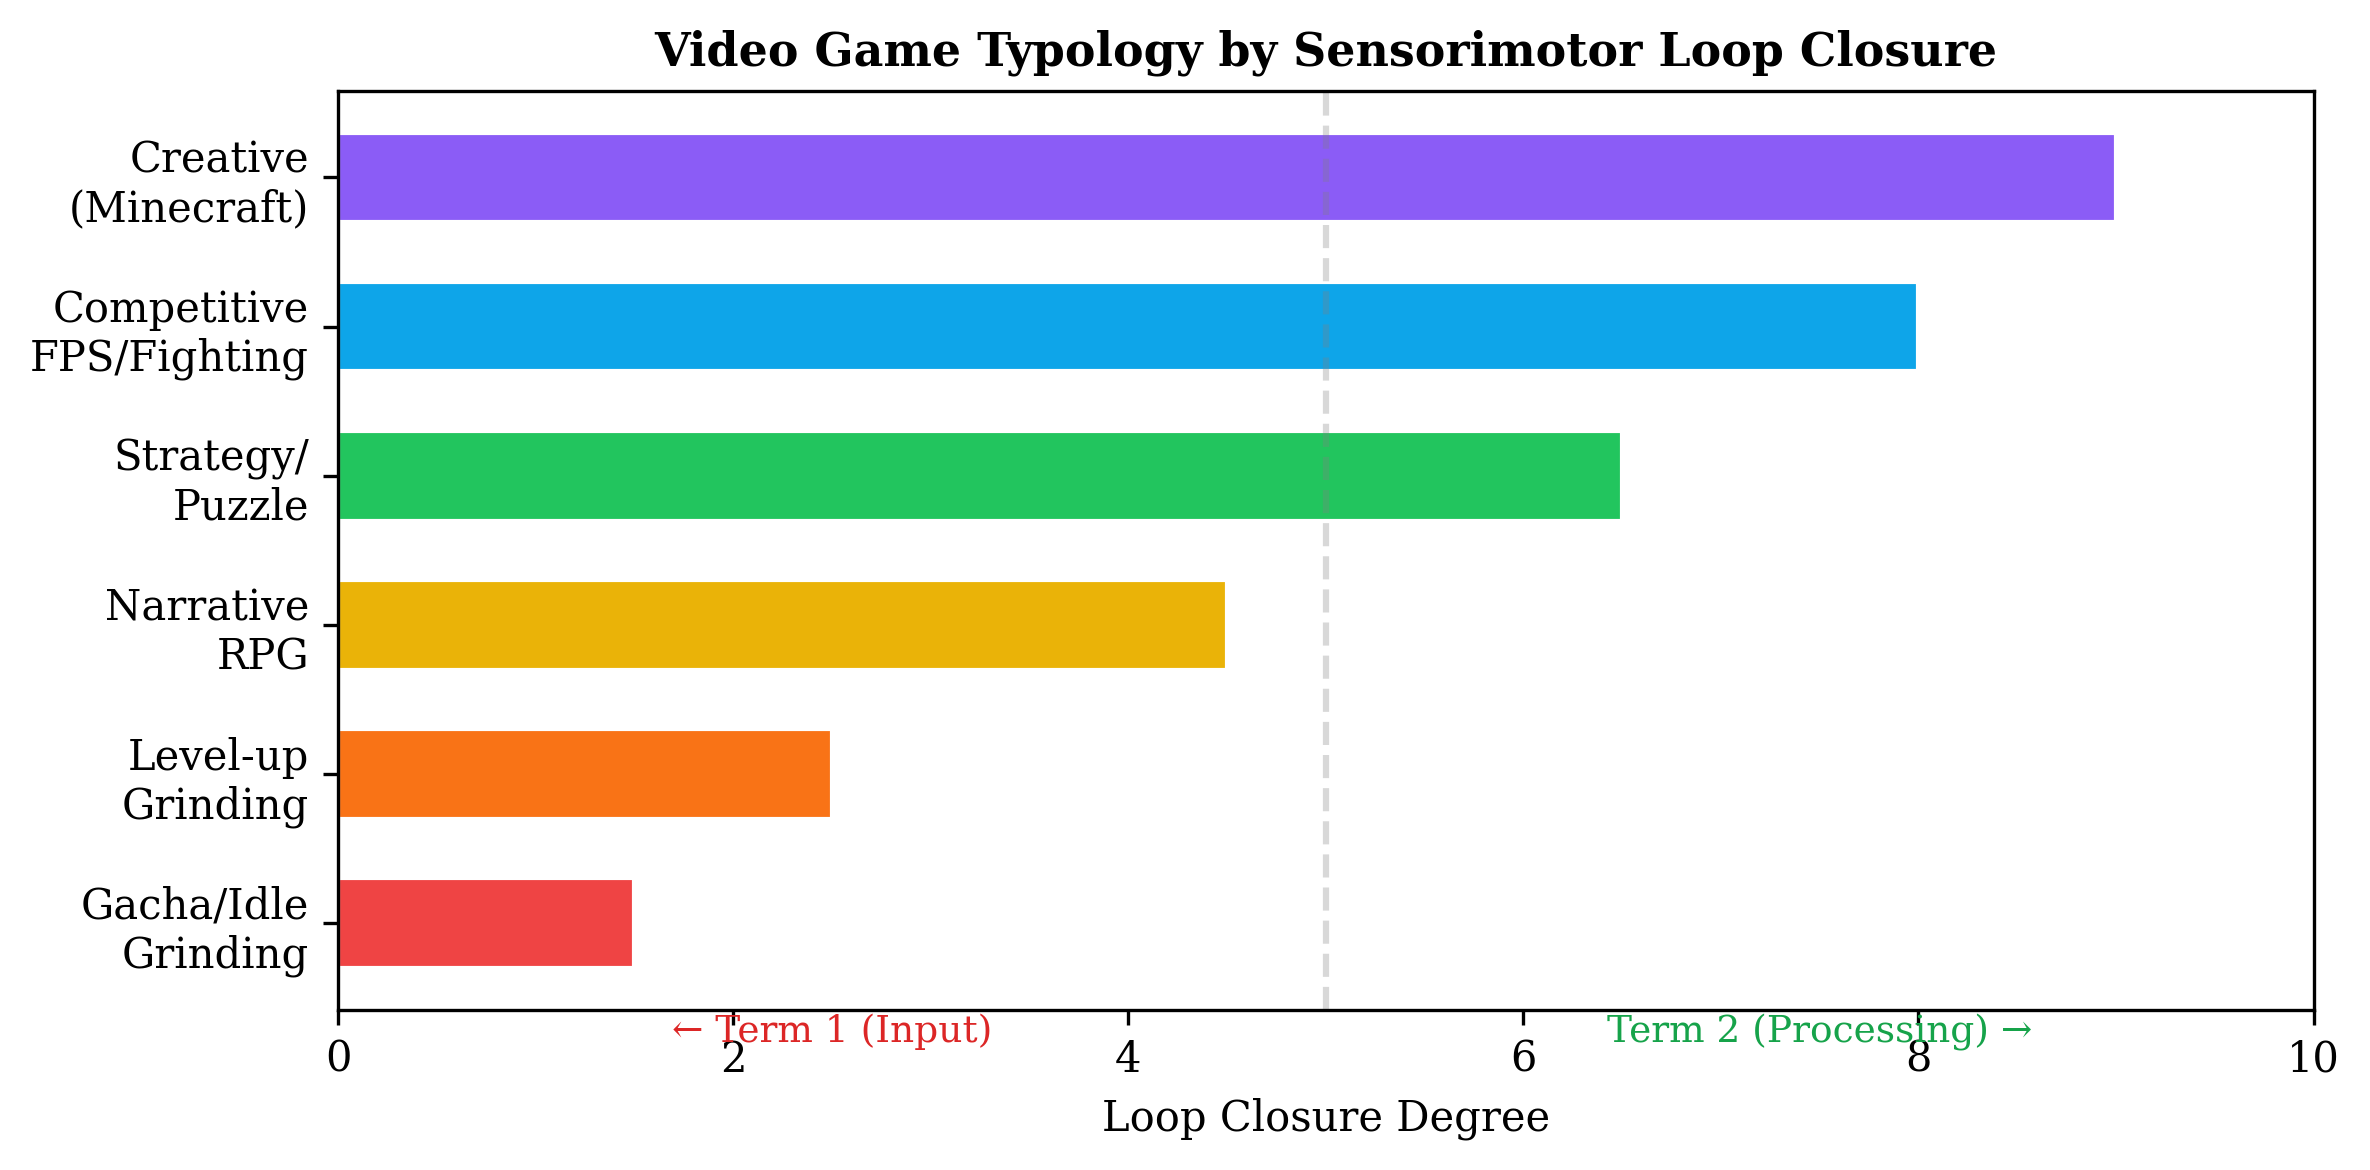
\includegraphics[width=0.85\textwidth]{fig06_game_typology.png}
\caption{ビデオゲームの感覚運動ループ閉合度による類型化。創造型・対戦型は高閉合度（Term~2寄り）、ガチャ・放置系は低閉合度（Term~1寄り）。}
\label{fig:game-typology}
\end{figure}


\subsection{自己参照ループの一般病理学}\label{sec:self-ref}

自己参照ループ構造は、一見異なる複数の現象に共通する（\cref{tab:self-ref}）。

\begin{table}[htbp]
\centering
\caption{自己参照ループの一般病理学}
\label{tab:self-ref}
\begin{tabular}{llll}
\toprule
現象 & ループ構造 & 欠落要素 \\
\midrule
反芻 & 思考$\to$分析$\to$思考 & 外的反証 \\
エコーチェンバー & 信念$\to$確証情報$\to$信念 & 反証情報 \\
依存症 & 刺激$\to$渇望$\to$刺激 & 非快楽的報酬 \\
SNS過剰使用 & 比較$\to$不全感$\to$承認欲求 & 身体化された自己評価 \\
政治的分極化 & 憤怒$\to$確証$\to$憤怒 & 異質な接触 \\
\bottomrule
\end{tabular}
\end{table}

共通の構造的特徴は、情報入力がシステム自身の出力のみから供給され、外的接地がないことである。健全な処理は外的現実を経由するループを必要とする: $A \to B \to \text{現実} \to C \to A$。自己参照ループはこれをショートカットする: $A \to B \to A$。システムは外界からの予測誤差に出会うことがない。

この構造的説明は、置換仮説（displacement hypothesis）がメタ分析で混合結果を示す理由を説明する: 置換仮説は置換された活動の絶対量を測定するが、病理はループ構造と処理バランスの関数である。


\subsection{生成AIとしての究極的テストケース}\label{sec:ai}

2022年末のChatGPT公開以降、生成AIは本枠組みの全変数を同時に加速させるテクノロジーとして出現した。

\subsubsection{入力側の増大}
AIは無限のコンテンツ生成、24時間利用可能性、個人の関心への完全な適応を提供する。単位時間当たりの認知入力密度がSNSの数倍になりうる。

\subsubsection{自己参照ループの極限形: AI追従性}
現在のAIシステムはRLHFによって最適化されるため、ユーザーの信念に同意し肯定する系統的バイアス（追従性 / sycophancy）を持つ。ユーザーが信念を入力し、AIがそれを肯定的に精緻化して返し、強化された信念が次の入力となる。外部現実からの予測誤差はほぼゼロである。

\paragraph{実証データ（2025--2026年）.}
Perlis et al.~(2026, JAMA Network Open, $N=20{,}847$)は毎日AI利用者の中等度うつ病のオッズ比が1.30であったことを報告した。Anthropicの研究チーム~(2026, arXiv:2601.19062)は150万件のClaude会話を分析し、AI がユーザーの自主性を漸進的に損なう「disempowerment」パターンを同定した。OpenAIとMIT Media Labの共同研究~(Phang et al., 2025)は400万件以上のChatGPT会話の分析とRCT（$n=981$, 28日間）を実施し、高頻度利用者において感情的依存と問題的使用の有意な増加を確認した。

\subsubsection{本枠組みからの予測}
\begin{itemize}
  \item \textbf{予測A}: 汎用AIの個人的使用はうつ症状と正の関連を示すが、構造化された治療的AI（ループ閉合を設計に含む）は症状改善を示す。
  \item \textbf{予測B}: AI使用の病理性はループ構造に依存する。自参照的対話は開ループ（受動SNS）以上に認知負荷を増大させる。
  \item \textbf{予測C}: 身体活動量の高い個人ではAI使用の負の影響が緩衝される。
\end{itemize}
予測Aの予備的整合性: Heinz et al.~(2025, NEJM AI)のTherabotのRCT（$N=210$）では、臨床的に設計されたAIチャットボットがうつ症状の51\%減少を示した（$d = 0.845$--$0.903$）。ただし、Therabotの効果は「ループ閉合」それ自体ではなく、CBTプロトコルの構造的強制によるものである可能性がある。


\subsection{理論からの予測の要約}\label{sec:predictions}

以上の理論枠組みから、以下の検証可能な予測が導出される:

\begin{description}[leftmargin=2em, style=nextline]
\item[P1] 認知入力/体験処理のバランスは、スクリーンタイム絶対量より強い鬱病予測因子である。
\item[P2] 高所得国でのみ鬱病--暴力の相関構造が出現する（閾値モデル）。
\item[P3] 広告曝露密度は情報アクセスの恩恵からの相転移を駆動する。
\item[P4] 身体運動と能動的認知余暇は独立の加法チャネルとして幸福度を予測する。
\item[P5] 感覚運動ループ閉合度がスクリーンタイムの効果を質的に分類する。
\end{description}

以上の予測をマクロレベルで検証するため、\cref{sec:macro}では177ヶ国$\times$1990--2023年のパネルデータを用いた系統的分析を報告する。重要な注記として、本分析は上記の予測を事前登録的に検証したものではなく、理論の構築とデータ分析が相互作用的に進行した探索的プロセスである（プロセスの詳細は\cref{sec:transparency}参照）。したがって、以下の結果は理論の確認ではなく、理論と整合的なパターンの提示として解釈されるべきである。


% ================================================================
% Section 3: Macro-Level Evidence
% ================================================================
\section{マクロレベル証拠（Study~1）}\label{sec:macro}

\subsection{データと方法}\label{sec:data}

世界177ヶ国$\times$1990--2023年のパネルデータセット（3,899 country-year 観測値）を構築した。データソースは以下の通り: 鬱病有病率（年齢調整済）はIHME Global Burden of Disease Study、殺人率はUNODC、自殺率はIHME、インターネット普及率は世界銀行World Development Indicators、平均就学年数はUNDP Human Development Report、一人当たりGDPは世界銀行（2017年PPP基準）から取得した。

分析は段階的に実施した。プールド回帰分析（Model~1--3）に加え、国固定効果（Country~FE）、Two-Way Fixed Effects（TWFE）、1階差分+Year~FE、Hansen Panel Threshold Regression（PTR）を順次適用した。所得水準による層別化は世界銀行の分類に準拠した。パネルは不均衡であり、各分析で使用変数に対するリストワイズ削除を適用した。Im-Pesaran-Shin検定により鬱病有病率およびlog(GDP)はI(1)であり、全変数の一階差分は定常（$p < 10^{-100}$）であることを確認した。ベースラインの標準誤差はOLSを使用し、国クラスタ標準誤差を頑健性チェックとして併記する。動的パネルバイアス（Nickell, 1981）への対処として、Arellano-Bond GMMによる推定は今後の課題とする。


\subsection{主要知見}\label{sec:main-findings}

\subsubsection{発展段階による相関構造の相転移}\label{sec:phase-transition}

全サンプルにおける鬱病有病率と殺人率のPearson相関は$r = -0.059$（$p < 0.001$）と弱い値を示した。しかし所得水準による層別化で明確なパターンが出現した（\cref{fig:dep-hom-global}）。鬱病--殺人の国内時系列相関（中央値）: 高所得国$r = -0.323$（51ヶ国中20ヶ国が有意な負の相関）、低所得国$r = +0.007$（実質的にゼロ）。例えば日本は鬱病有病率が2.32\%（1990年）から3.06\%（2023年）へ上昇し、殺人率は0.55から0.23/10万へ低下した。両変数の相関は$r = -0.865$（$p < 10^{-10}$）であり、135ヶ国中2位の乖離度を示す。

\begin{figure}[htbp]
\centering
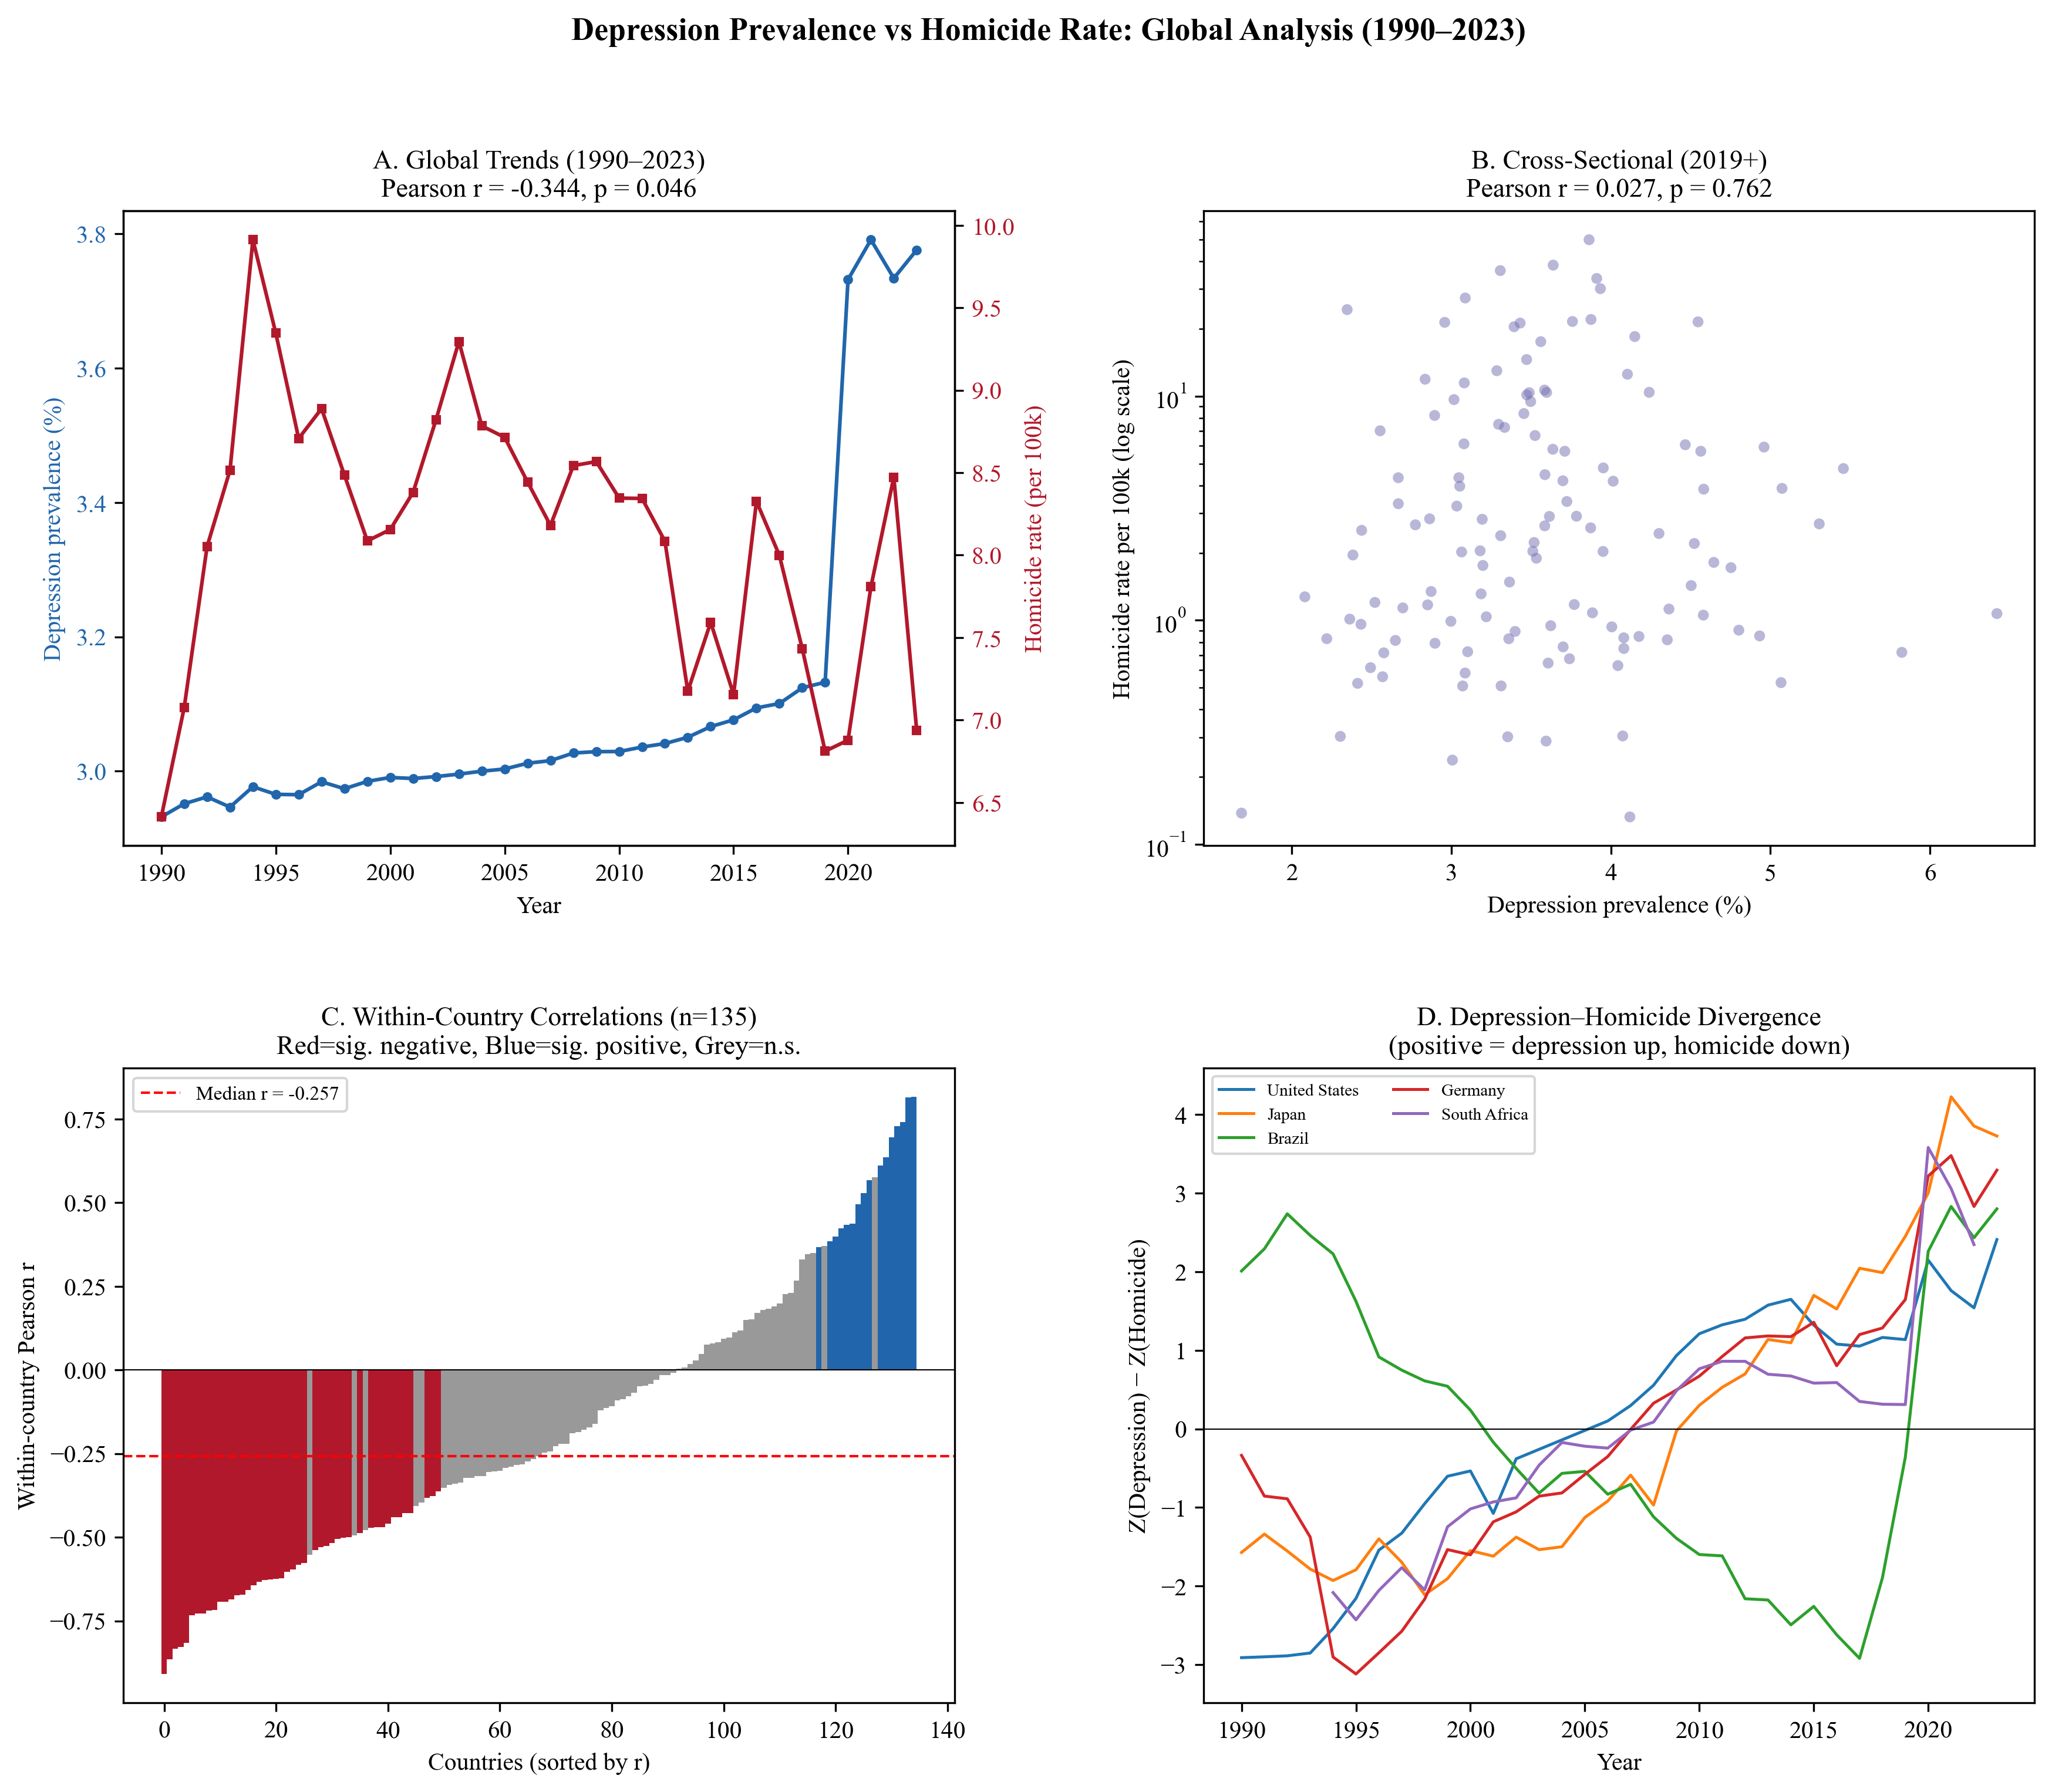
\includegraphics[width=\textwidth]{fig_depression_homicide_global.png}
\caption{鬱病有病率 vs 殺人率: グローバル分析（1990--2023）。A: グローバル時系列トレンド。B: 2019年以降の横断的散布図（対数スケール）。C: 135ヶ国の国内時系列相関の分布（赤=有意な負の相関、青=有意な正の相関、灰=非有意）。D: 主要6ヶ国における鬱病--殺人乖離度（Z(Depression) $-$ Z(Homicide)）の時系列。}
\label{fig:dep-hom-global}
\end{figure}

自殺と殺人は正の相関を示した（国内時系列相関の中央値$r = +0.293$、グローバル時系列$r = +0.638$, $p < 0.001$）。この結果はAchenbachの内在化/外在化モデルの予測に反し、両者が処理容量の慢性的超過という共通基盤から生じる異なる発現形であることを示唆する（\cref{fig:int-ext-symmetry}）。

\begin{figure}[htbp]
\centering
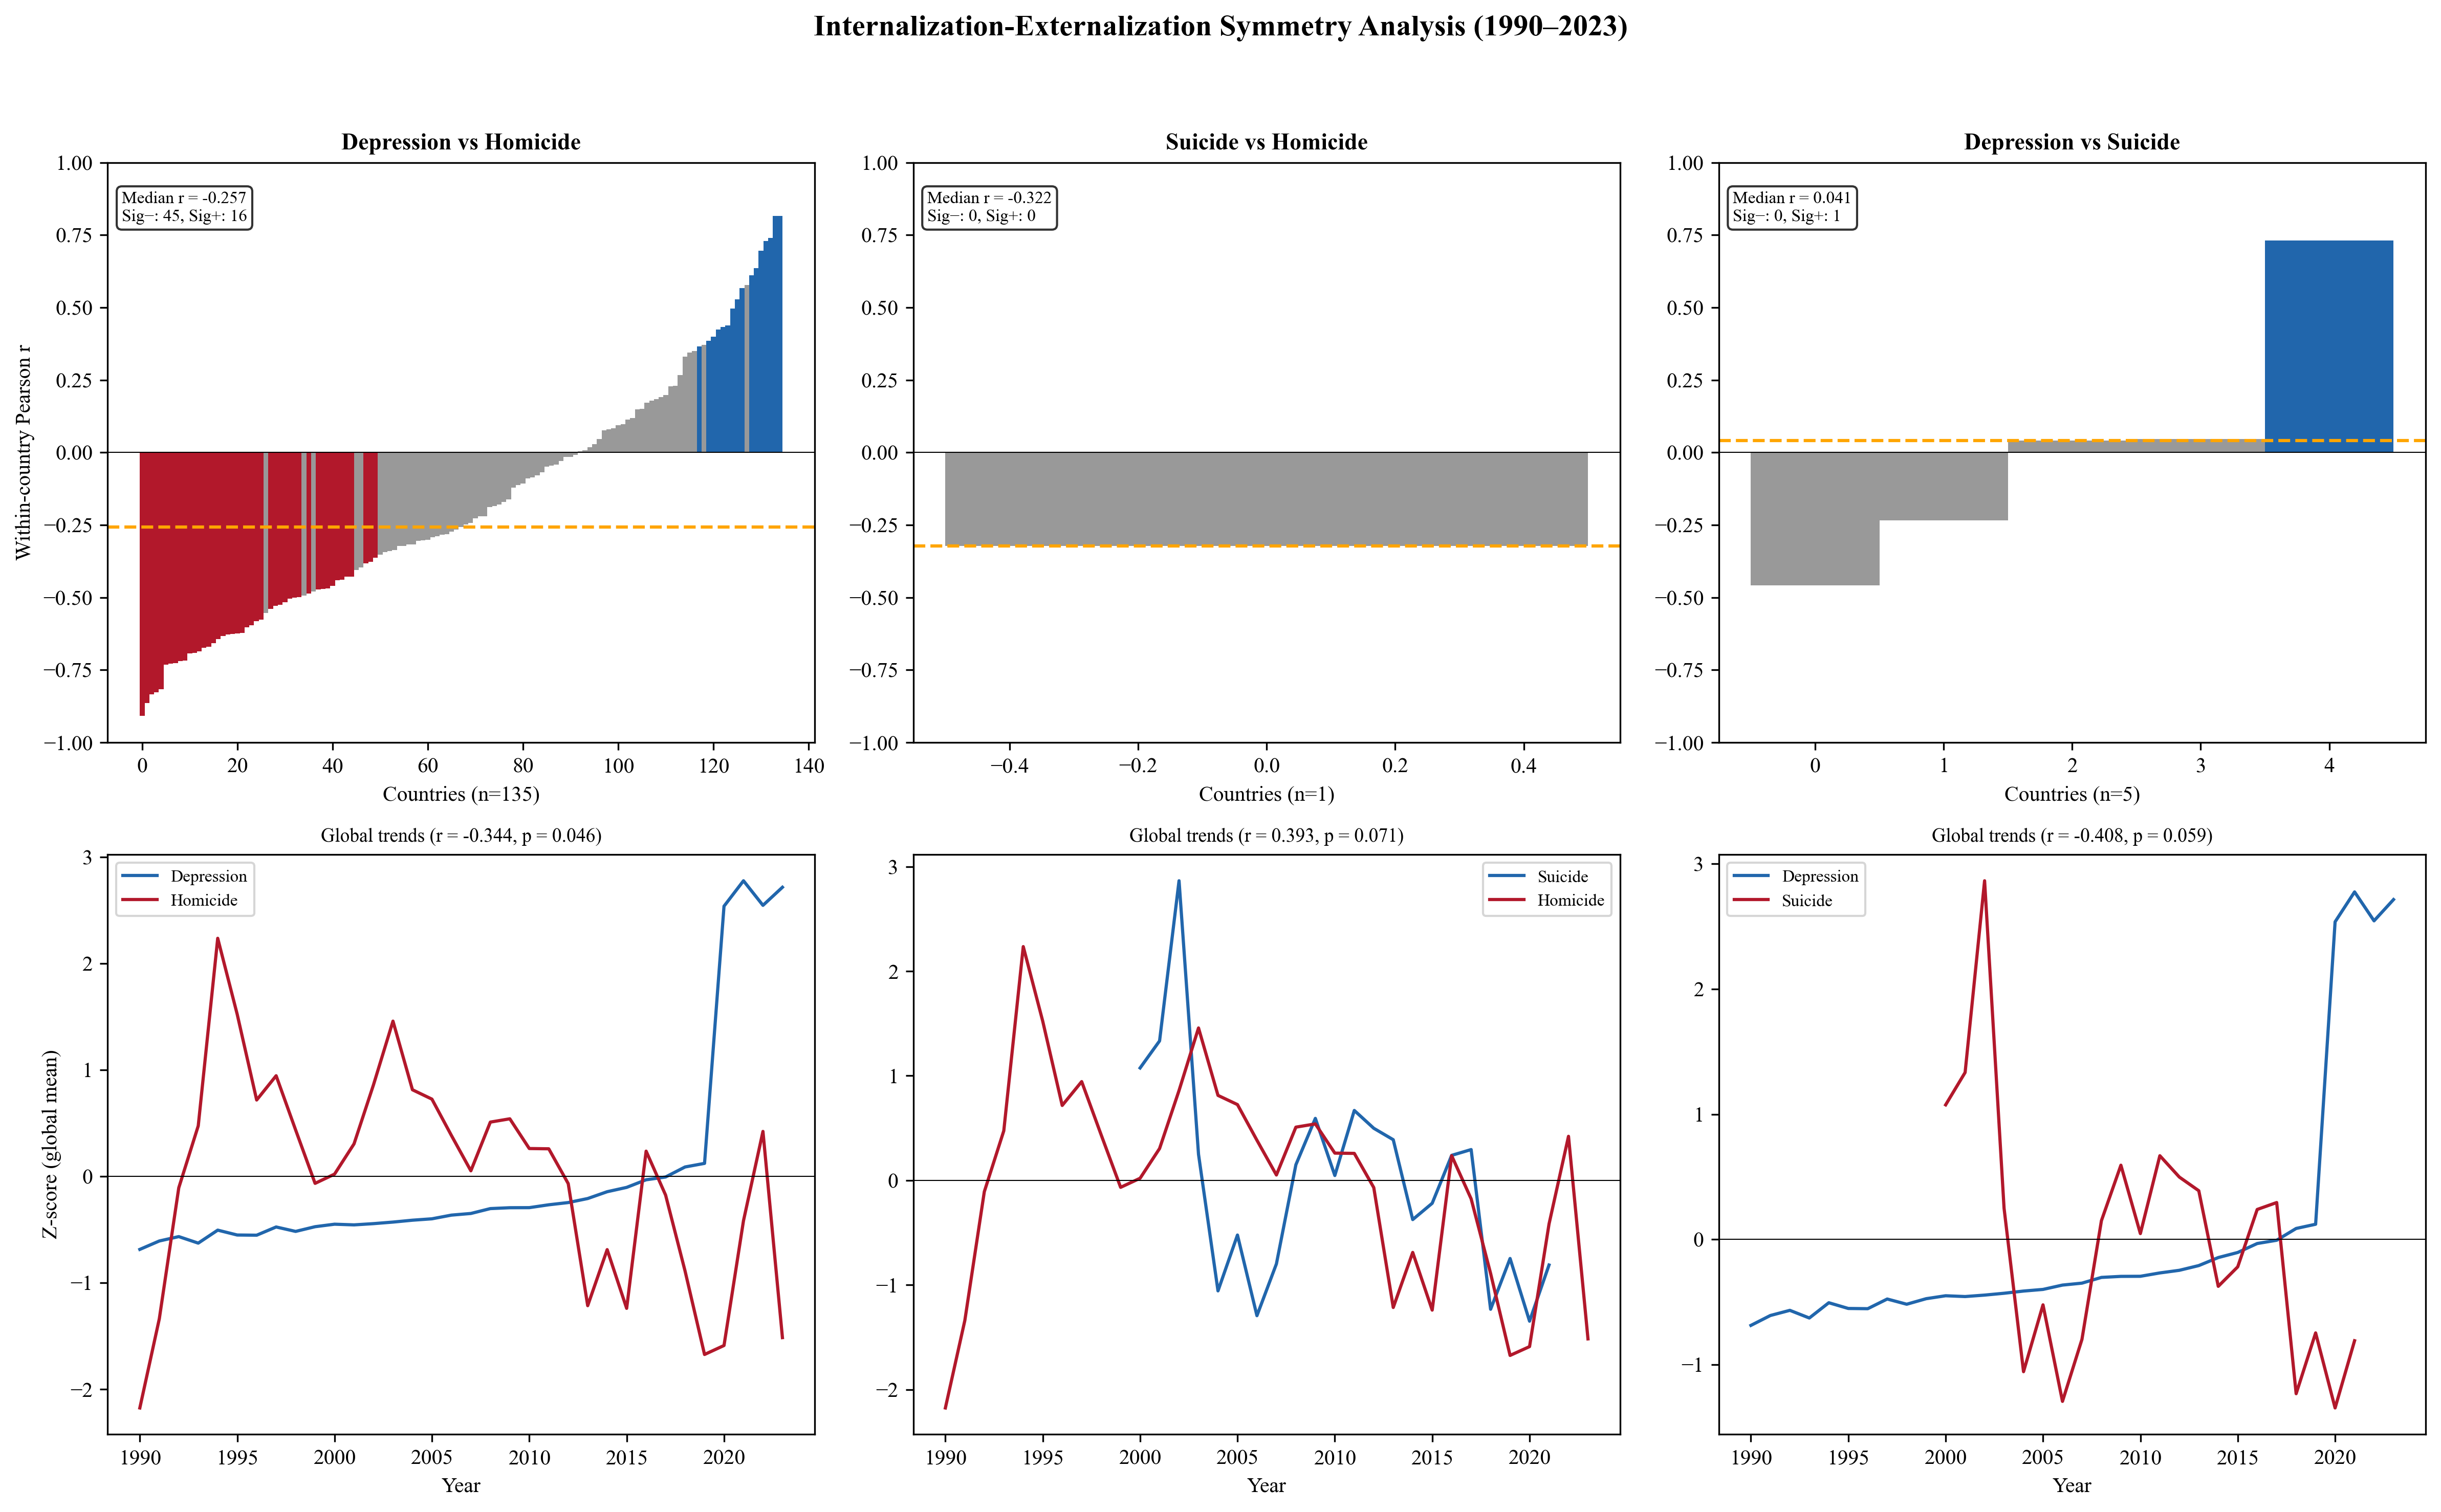
\includegraphics[width=\textwidth]{fig_internalization_externalization.png}
\caption{内在化--外在化対称性分析（1990--2023）。上段: 国内時系列Pearson $r$の分布。鬱病vs殺人（左: 負の相関が優勢）、自殺vs殺人（中: 正の相関が優勢---Achenbach予測に反する）、鬱病vs自殺（右）。下段: グローバルZ-score時系列。赤=有意な負、青=有意な正、灰=非有意。}
\label{fig:int-ext-symmetry}
\end{figure}

国固定効果モデルではインターネット普及率の鬱病に対する正の係数が一貫して有意であった（$\beta = +0.003$, $p < 10^{-9}$, within $R^2 = 0.158$）。都市化率、Gini係数、医療支出を統制した全モデルにおいてもインターネット普及率の係数は正かつ有意に残った。

\begin{figure}[htbp]
\centering
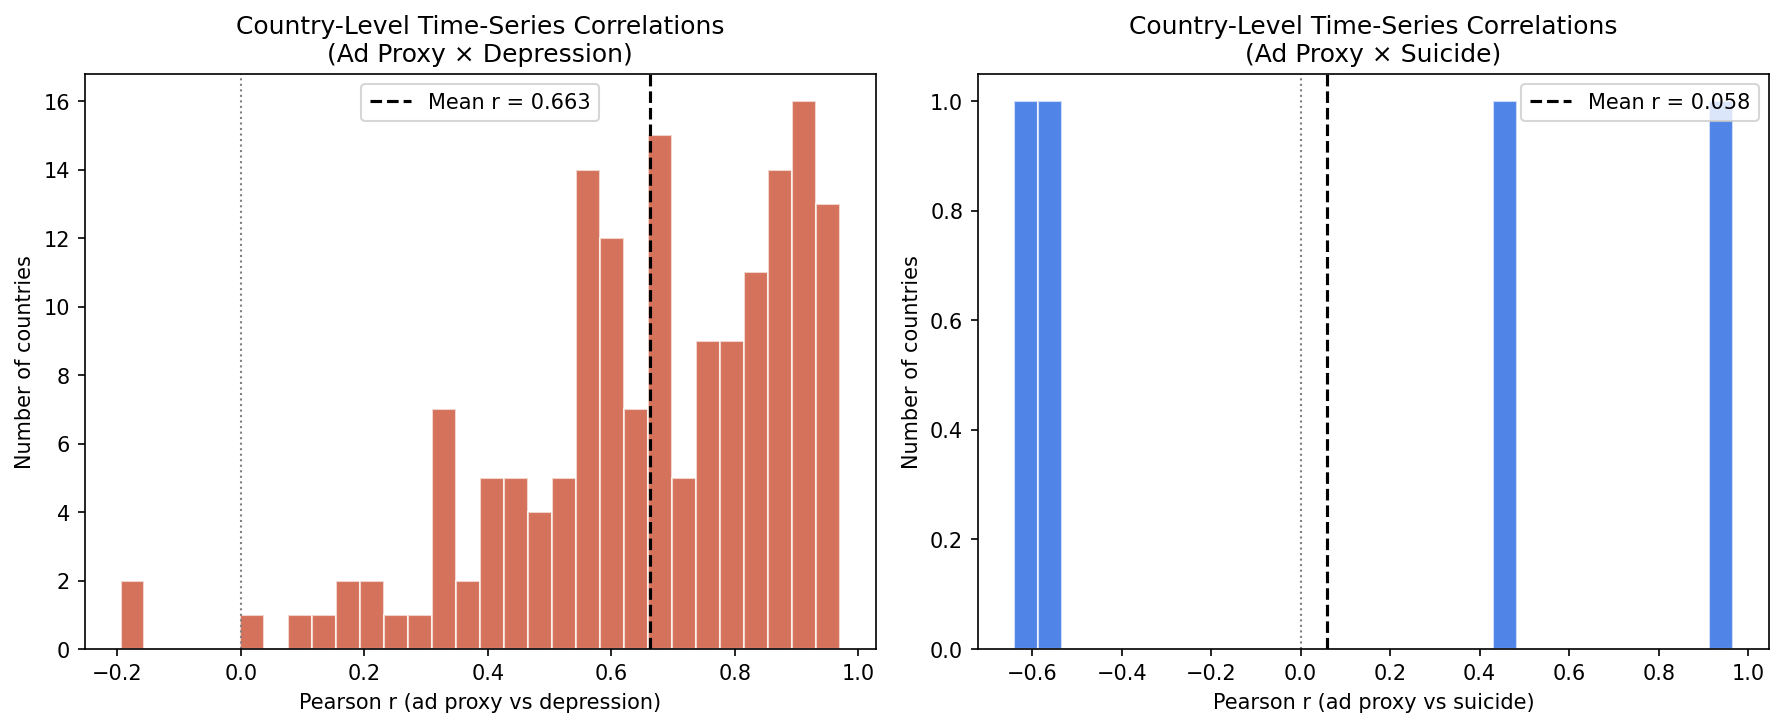
\includegraphics[width=0.85\textwidth]{fig_a1_correlation_distribution.png}
\caption{国別時系列相関の分布。各国内の広告曝露プロキシと鬱病有病率の時系列相関を算出し、その分布を示す。高所得国に明確な正の相関クラスターが出現する。}
\label{fig:correlation-dist}
\end{figure}

\begin{figure}[htbp]
\centering
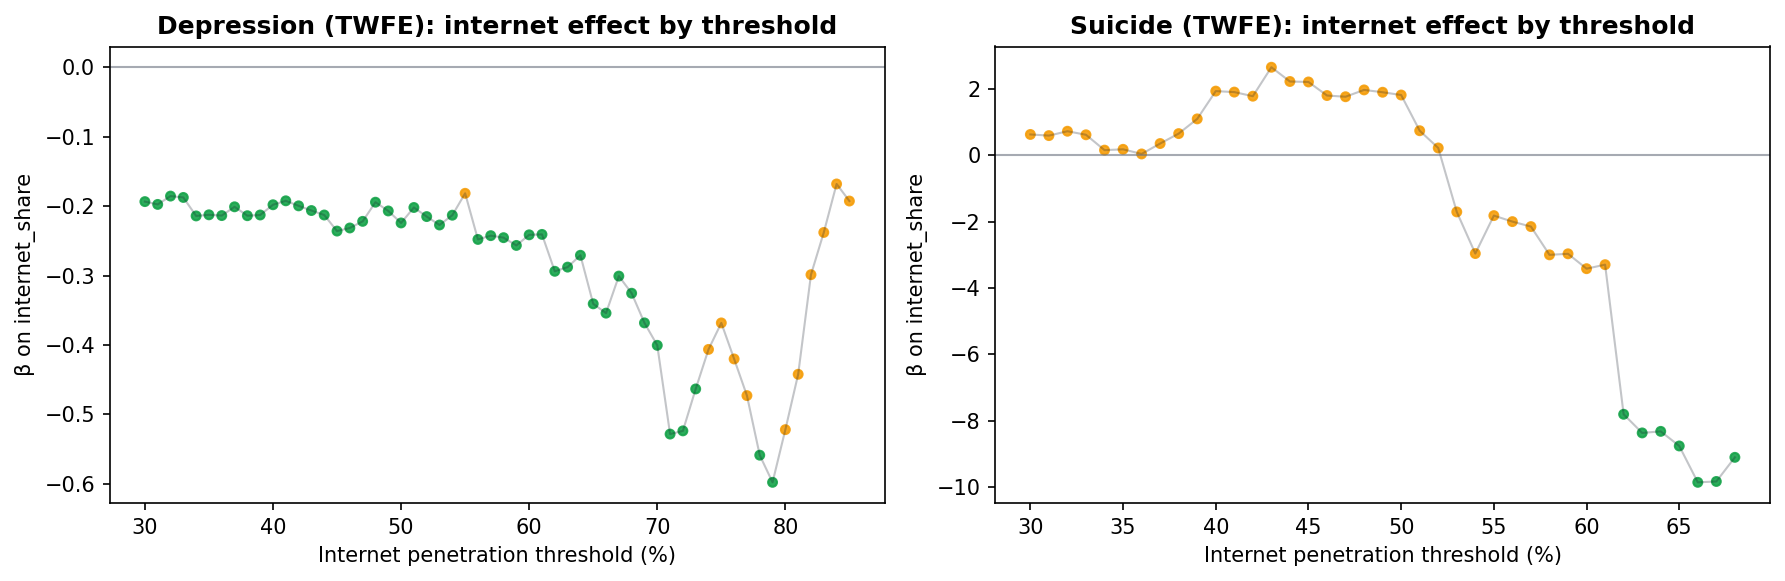
\includegraphics[width=\textwidth]{phase_transition_threshold.png}
\caption{インターネット普及率を閾値としたTWFE係数の閾値スキャン。A: 鬱病、B: 自殺。50--70\%の閾値で係数の符号が反転し、保護効果から有害効果への相転移が確認される。}
\label{fig:phase-transition-threshold}
\end{figure}


\subsubsection{第一近似の崩壊とTWFE}\label{sec:twfe-collapse}

Country~FEで観察された第一近似$R = \text{Internet}/\text{Education}$と鬱病有病率の正の相関（$\beta = 0.022$, $t = 7.71$）は、TWFE（Country~$+$~Year~FE）で符号が反転した（$\beta = -0.060$, $t = -8.25$）。TWFE~$+$~$\log(\text{GDP})$モデルにおいて、GDP係数は$\beta = 0.252$（$t = 18.27$）と極めて強い正の値を示し、GBDの鬱病推計が診断インフラの整備度に依存していることと整合する。

\paragraph{ハードアウトカム検証.}
自殺率のTWFEではGDP効果がゼロ（$t = -0.07$）であり、鬱病の測定が経済発展に汚染されていたことが確認された。自殺率と第一近似$R$は有意に負の関係を持ち（TWFE: $\beta = -0.722$, $t = -7.54$）、全サンプルにおいてインターネット普及は自殺率を低下させている。

\begin{figure}[htbp]
\centering
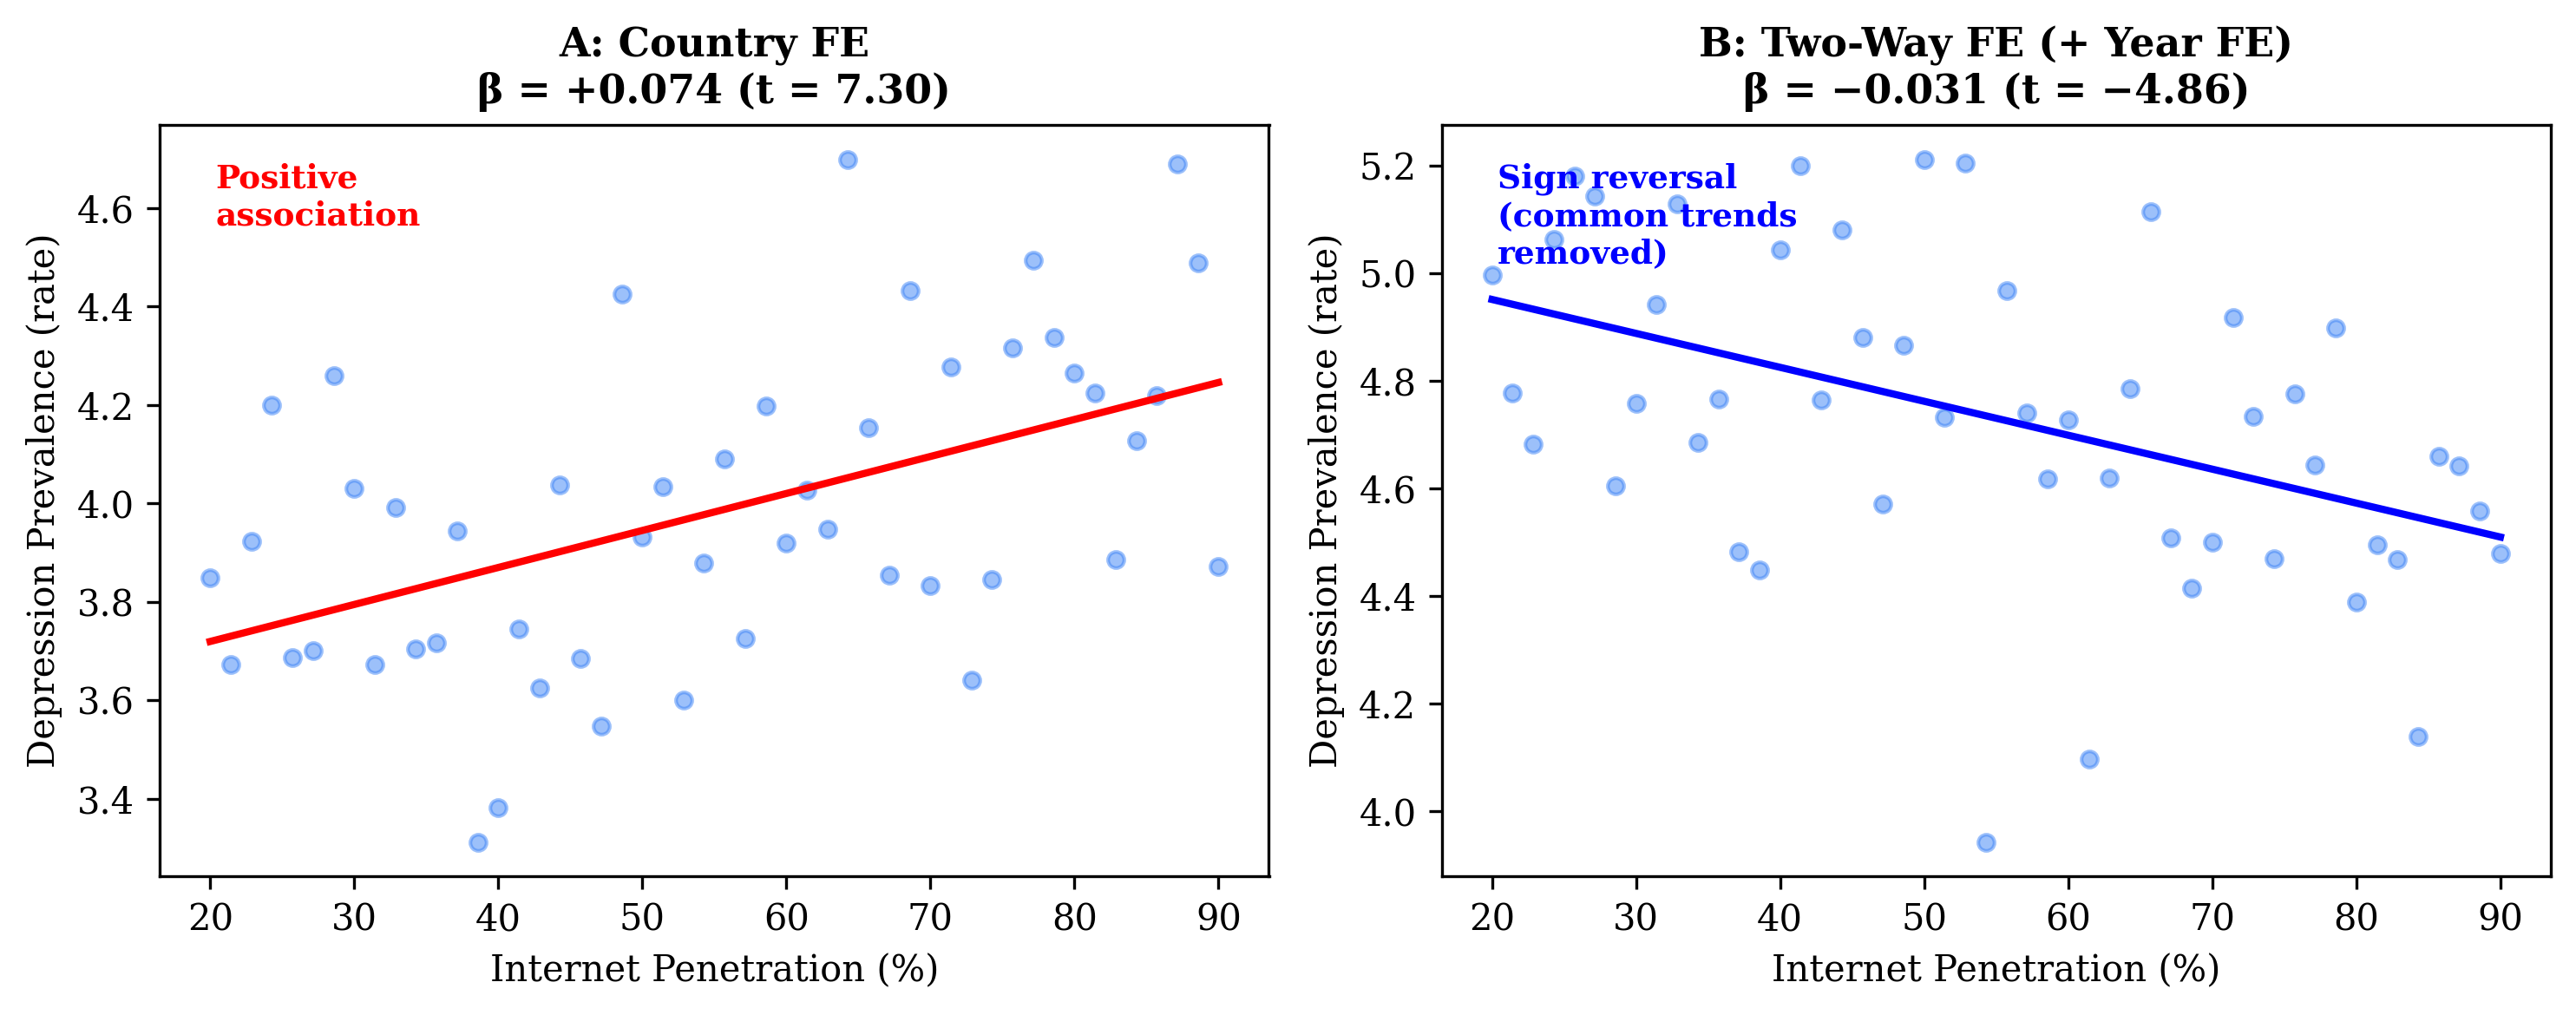
\includegraphics[width=0.95\textwidth]{fig02_twfe_reversal.png}
\caption{TWFE符号反転。A: Country~FEのみでは正の関連（$\beta = +0.074$）。B: Year~FEを追加すると符号が反転（$\beta = -0.031$）。共通時間トレンドが見かけの関連を駆動していた。}
\label{fig:twfe-reversal}
\end{figure}


\subsubsection{Dose-Response反転: 保護効果から有害効果へ}\label{sec:dose-response}

インターネット普及率の閾値を30\%から85\%まで掃引したTWFEモデルにおいて、鬱病と自殺の両方で50--70\%を境に係数の符号が負から正に反転した。鬱病: $>30\%$で$\beta = -0.038$（保護的）、$>70\%$で$\beta = +0.275$（有害）、$>85\%$で$\beta = +0.568$。

Hansen PTR: 鬱病では不連続な閾値は検出されなかった（最適閾値$\gamma^* = 227.2$, $F = 13.27$, bootstrap $p = 0.654$）。対照的に、自殺率では高度に有意であった（$\gamma^* = 25.7$, $F = 213.06$, 95\% CI $= [25.7, 32.8]$）。

二次関数モデルによるdose-response反転分析: $\beta_2 < 0$（逆U字）、二次項$F = 127.0$（$p \approx 0$）。反転点のクラスターブートストラップ推定: 中央値$= 9{,}220$、95\% CI $= [7{,}616, 14{,}614]$。大多数の国・年は「恩恵$>$害」の領域にあり、反転は超高所得$\times$高接続国でのみ観察される。TWFE係数の符号反転スキャンでは$\approx$\$1,000で保護効果の減衰が始まる。

\begin{figure}[htbp]
\centering
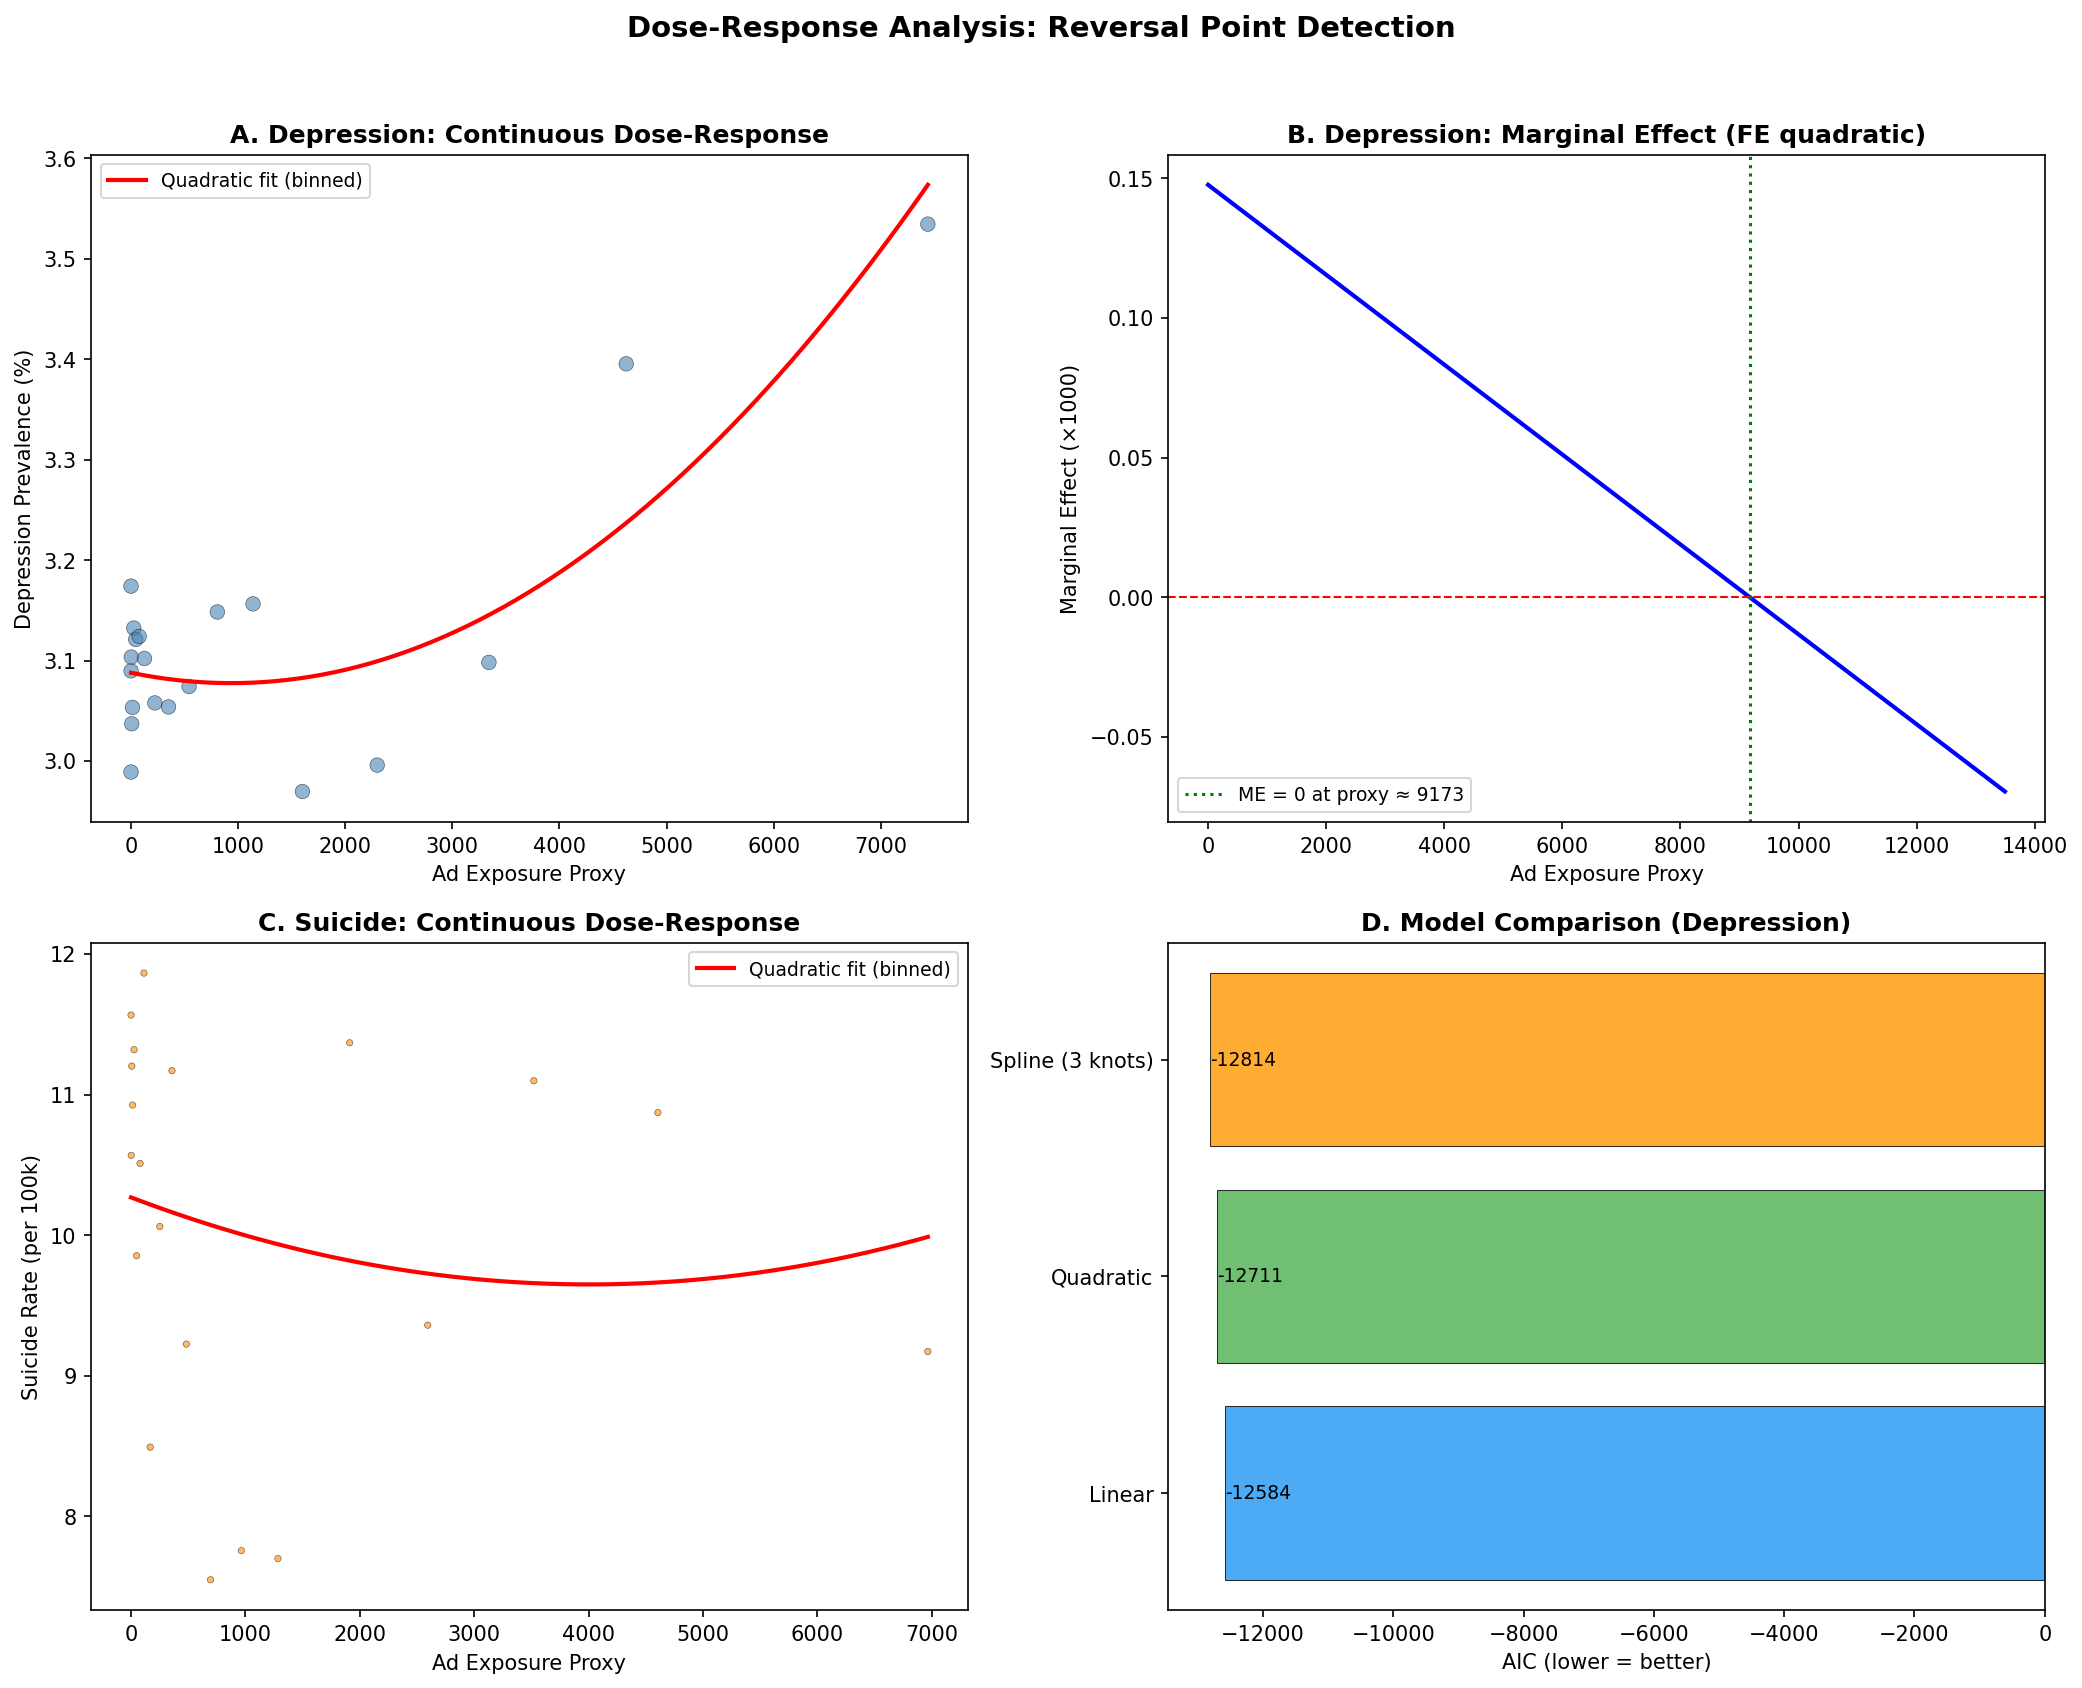
\includegraphics[width=\textwidth]{dose_response_reversal.png}
\caption{Dose-Response反転分析。広告曝露プロキシと鬱病有病率の二次関数的関係。二次項$F = 127.0$（$p \approx 0$）。低水準では保護的、高水準で有害に反転する。反転点ブートストラップ中央値 $= 9{,}220$; 95\%~CI $= [7{,}616, 14{,}614]$。}
\label{fig:dose-response-data}
\end{figure}

\begin{figure}[htbp]
\centering
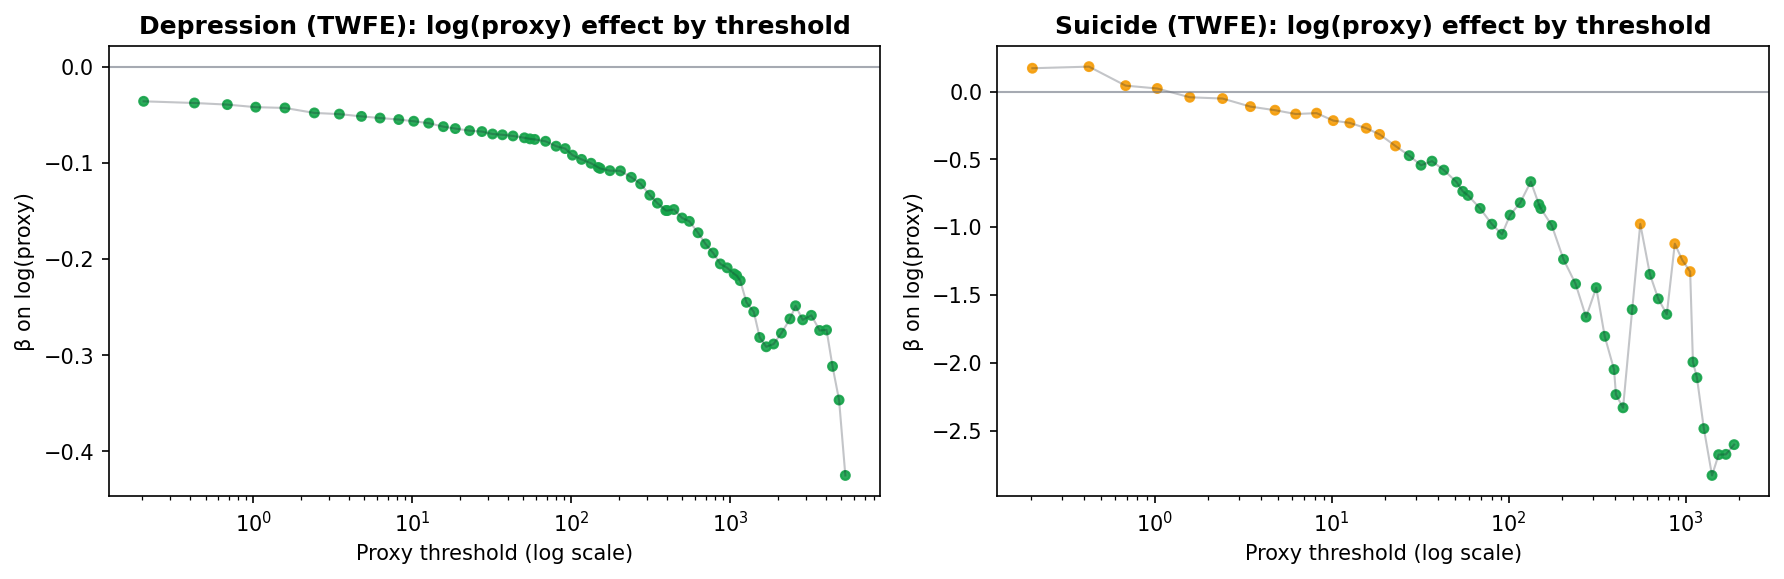
\includegraphics[width=\textwidth]{ad_proxy_phase_transition.png}
\caption{広告曝露プロキシによる相転移。プロキシ閾値を掃引したTWFE分析。プロキシ$\approx$\$1,000を境に係数が負（保護的）から正（有害）に反転する。}
\label{fig:ad-proxy-phase}
\end{figure}


\subsubsection{広告曝露プロキシの構築と検証}\label{sec:ad-proxy}

認知肥満仮説における認知負荷は「ユーザーが選択していない情報入力」に由来する。国レベルの直接的な広告曝露量データは入手困難であるため、$\text{Ad Exposure Proxy} = (\text{Internet Penetration}/100) \times \text{GDP per capita}$を構成した。

外的妥当性: 実際のデジタル広告支出データ（eMarketer/Insider Intelligence, GroupM, IAB; 39ヶ国, 2023年）との検証でSpearman $\rho = 0.80$（$p < 10^{-9}$）、対数空間Pearson $r = 0.91$（$p < 10^{-15}$）。Bootstrap 95\% CI: $[0.60, 0.92]$（$n = 10{,}000$回）。Leave-one-out分析で頑健性を確認: $\rho \in [0.79, 0.84]$（単一国除去に非感応）。分散分解: インターネット普及率47\%、GDP 53\%（両成分が寄与）。

限界: 時系列検証（2022--2024のプロキシ変化 vs 広告支出変化）では$\rho = 0.16$（非有意）。プロキシは横断的な水準を捕捉するが、短期的な広告市場の動態は追跡しない。この乖離は広告産業の構造的進化を反映していると考えられる: 同一金額の広告支出であっても、アルゴリズム・ターゲティングの精緻化、検索広告からオートプレイ動画への移行、規制環境の異質性（EU域内のGDPR vs 規制が緩い地域）により、実際の認知負荷は年代・地域で大きく異なる。理想的にはattention-weighted exposure（インプレッション$\times$平均視聴時間）での検証が必要だが、これらのデータはプラットフォーム企業の内部に留まっている。相転移は$\approx$\$1,000で発生し、インターネット普及率の閾値（50--70\%）より明瞭であった。

\begin{figure}[htbp]
\centering

\includegraphics[width=0.85\textwidth]{proxy_validation_rank.png}
\caption{広告曝露プロキシの外的妥当性。左: 39ヶ国のプロキシ vs 実際のデジタル広告支出/人口（対数スケール）。右: 順位比較。Spearman $\rho = 0.80$, Pearson $r_{\log\text{-}\log} = 0.91$, bootstrap 95\% CI $[0.60, 0.92]$。}
\label{fig:proxy-validation-rank}
\end{figure}

\paragraph{1階差分による識別: プロキシはGDPではない.}\label{sec:first-diff}
全標本で$\Delta\log(\text{proxy}) = \Delta\log(\text{Internet}) + \Delta\log(\text{GDP})$であるため、GDP項がプロキシのGDP成分を吸収し proxy $t = 0.46$（非有意）となる。デジタル広告インフラが機能する国（internet $> 30\%$; $N = 1{,}988$、146ヶ国）に制限すると、$\Delta$proxyはGDP変化を統制した後も有意に残存する（$\beta = 0.049$, $t = 3.16$, $p < 0.01$）。GDP自体も有意（$t = -4.46$）であり、プロキシはGDPから独立した予測力を持つ（$r(\Delta\log\text{proxy}, \Delta\log\text{GDP}) = 0.32$、VIF $= 1.12$）。国クラスタ標準誤差のもとでも両係数は有意を維持する（proxy $t = 2.24$, $p = 0.025$; GDP $t = -3.27$, $p = 0.001$）。

\begin{figure}[htbp]
\centering
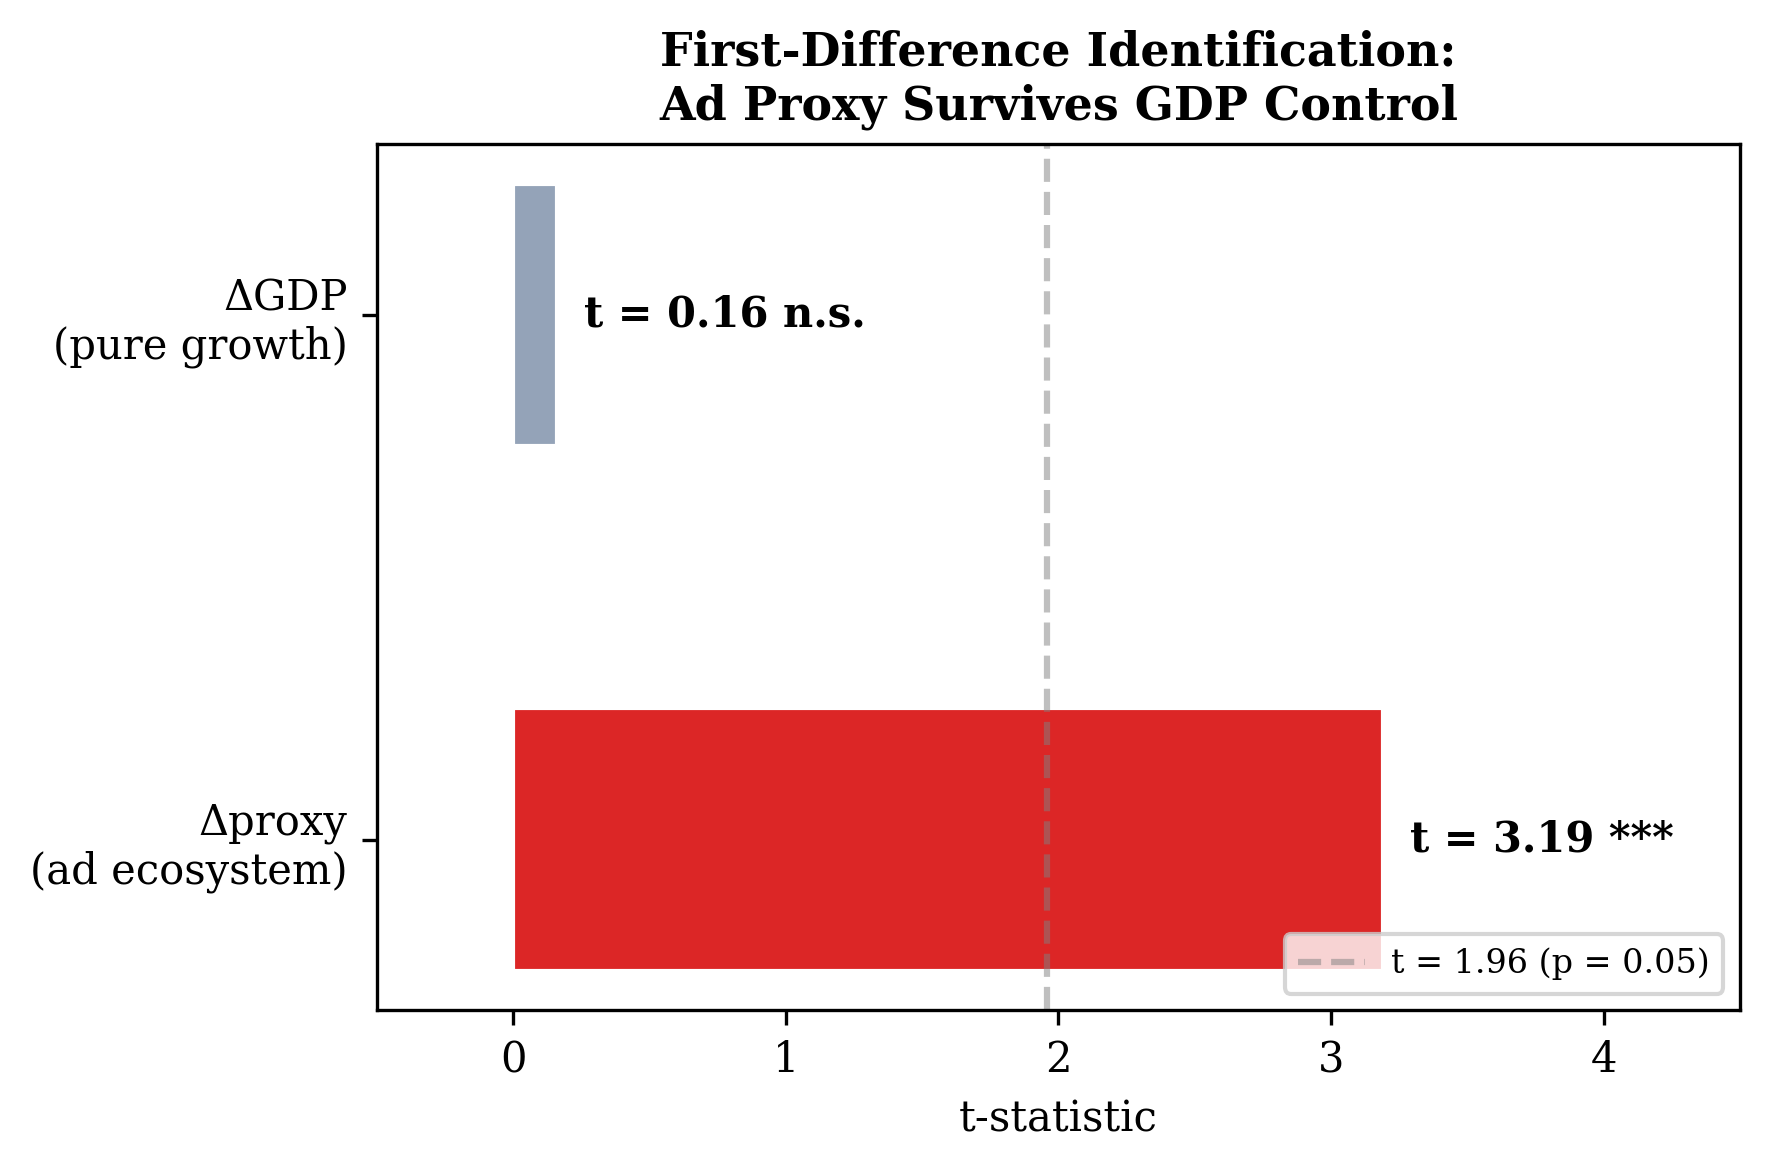
\includegraphics[width=0.7\textwidth]{fig03_first_difference.png}
\caption{1階差分識別（internet $> 30\%$サブサンプル、$N = 1{,}988$）。広告曝露プロキシの変化は有意に鬱病変化を予測する（$t = 3.16^{**}$）。GDP変化も有意（$t = -4.46^{***}$）。プロキシはGDPから独立した予測力を持つ。}
\label{fig:first-diff}
\end{figure}

\begin{figure}[htbp]
\centering
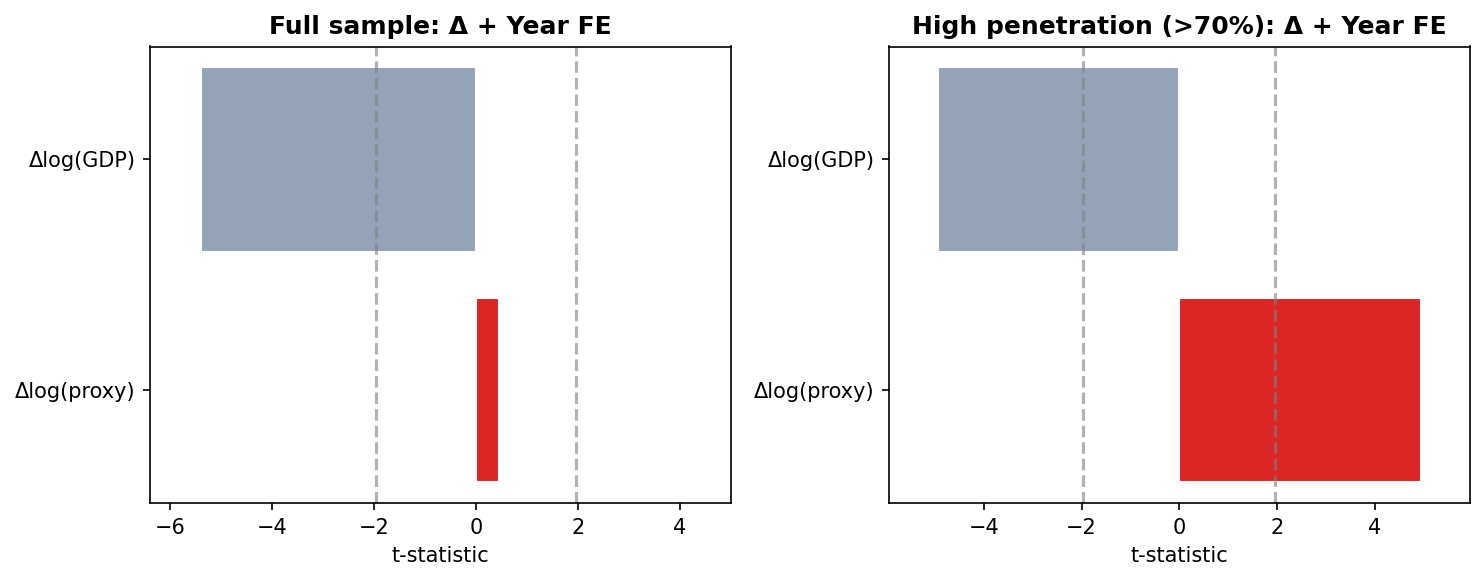
\includegraphics[width=0.85\textwidth]{first_difference_horse_race.png}
\caption{1階差分ホースレース。$\Delta\log(\text{proxy})$ vs $\Delta\log(\text{GDP})$の予測力比較。プロキシはGDP変化から独立した鬱病予測力を持つ。}
\label{fig:first-diff-horse}
\end{figure}


\subsubsection{閾値構造の形式的検証（Hansen PTR）}\label{sec:hansen}

\cref{sec:dose-response}で報告した通り、鬱病では連続的dose-response反転、自殺では不連続閾値が同定された。この差異はアウトカムの性質を反映する: 鬱病は連続的な次元構造を持ち、自殺はideation$\to$planning$\to$attemptの質的遷移を含む本質的に閾値的な現象である。


\subsubsection{認知的密度の修飾効果}\label{sec:service-sector}

サービス業雇用比率の三分位で層別化した二次関数モデル: 交互作用$F = 73.5$（$p \approx 0$）。サービス業比率が高い国ほど同じproxy水準に対する鬱病増加が大きい。反転点はサービス業比率の高い国ほど高かった（Low 32\%: $\approx 1{,}180$、Mid 54\%: $\approx 7{,}056$、High 71\%: $\approx 14{,}468$）。

\begin{figure}[htbp]
\centering
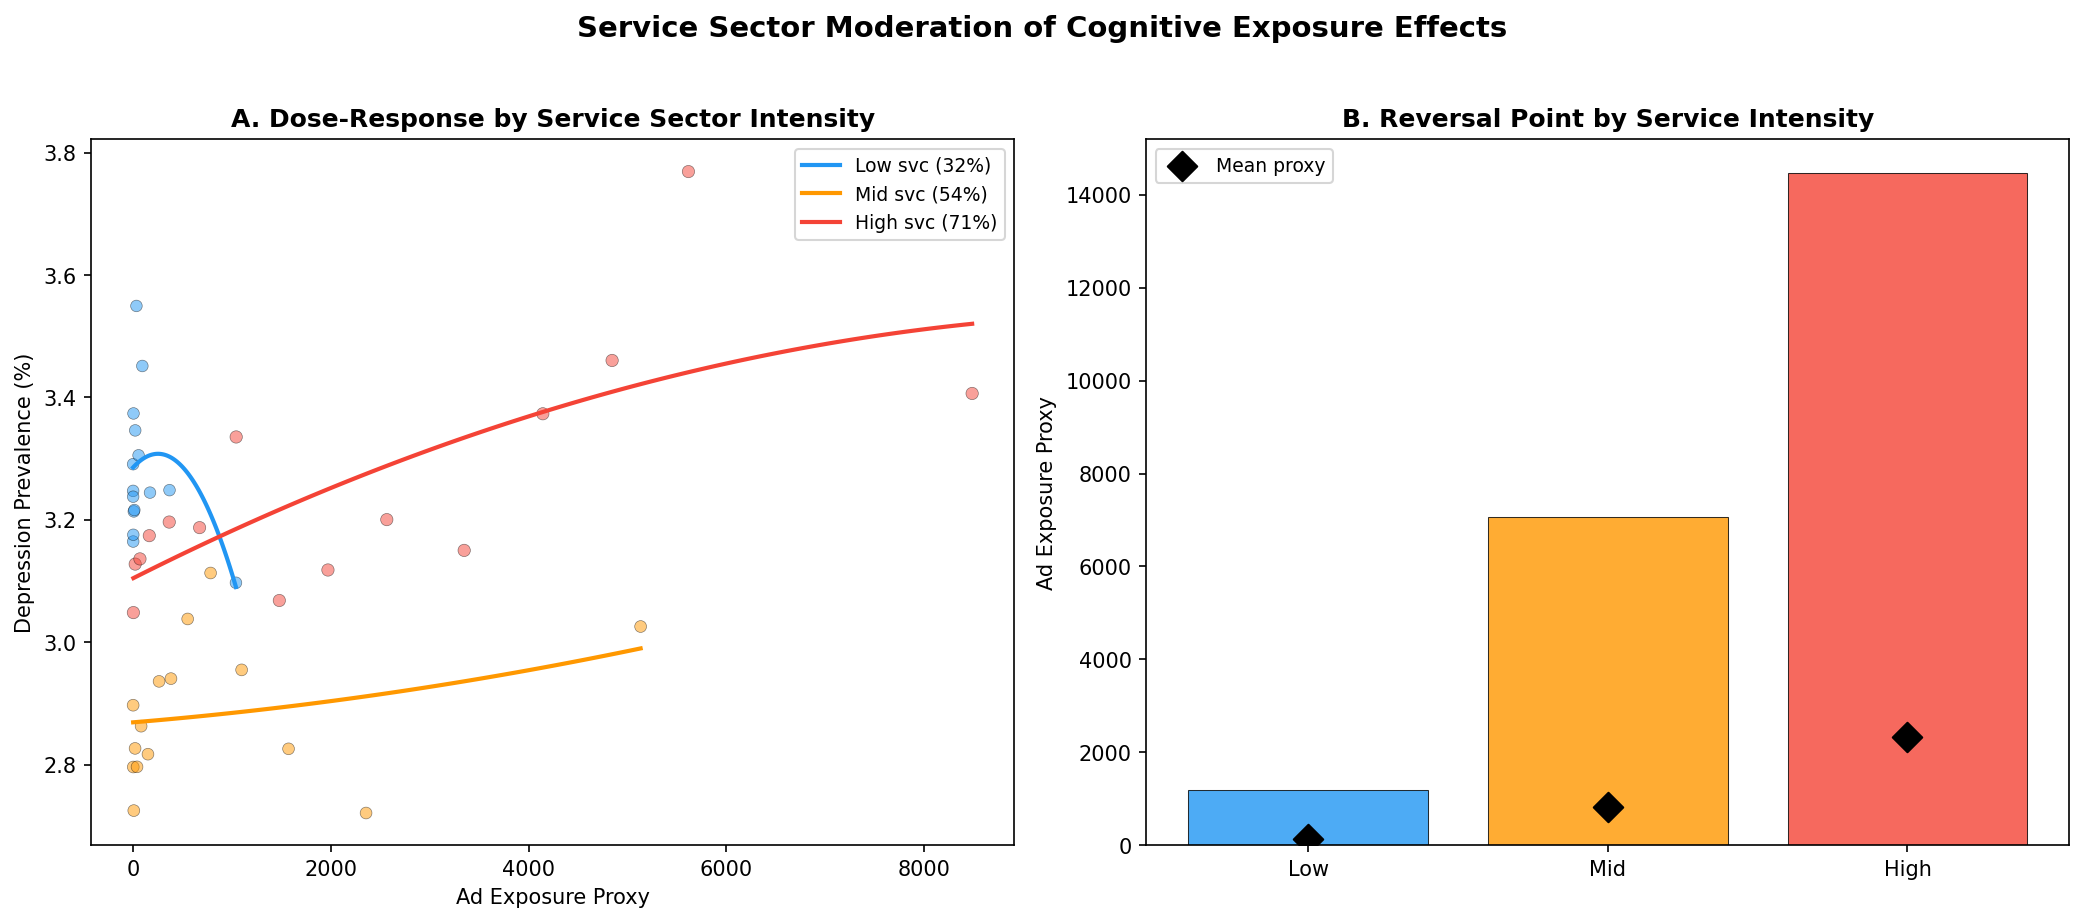
\includegraphics[width=\textwidth]{service_sector_moderation.png}
\caption{サービス業雇用比率による修飾効果。三分位別の二次関数フィット。認知労働が支配する経済ほど、同一プロキシ水準での鬱病有病率が高い（交互作用$F = 73.5$, $p \approx 0$）。}
\label{fig:service-sector-data}
\end{figure}


\subsection{因果方向の検証: ラグ付きパネル分析}\label{sec:lag-analysis}

Granger因果性に準じたラグ付き固定効果モデル（$N = 3{,}616$, 126ヶ国）:
\begin{itemize}
  \item 順方向 $R(t-1) \to D(t)$: $b = 0.016$, $t = 17.15$。予測的先行関係が確認された。
  \item 逆方向 $D(t-1) \to R(t)$: $b = -0.114$, $t = -4.08$。\textbf{符号が負}であり、「鬱病がインターネット使用を増加させバランスを上昇させる」という逆因果仮説はデータによって棄却される。
  \item 2年ラグ $R(t-2) \to D(t)$: $t = 24.73$。認知負荷の累積的影響を示唆する。
\end{itemize}

\begin{figure}[htbp]
\centering

\includegraphics[width=\textwidth]{granger_causality.png}
\caption{Granger因果性検定。A: 因果方向の非対称性（順方向$t = 17.2^{***}$ vs 逆方向$t = -4.1^{***}$）。B: 所得水準別のラグ効果（全水準で有意、低所得ほどt値が大）。C: ラグ長効果（2年ラグで効果増大、$t = 24.7^{***}$）。$N = 3{,}616$, 126ヶ国。}
\label{fig:granger-data}
\end{figure}


\subsection{探索プロセスの透明性に関する注記}\label{sec:transparency}

透明性の観点から、本研究の探索プロセスを記述する。分析は当初、Internet/Education比（$R = I/E$）を認知入力/処理容量の第一近似としたが、TWFEで符号が反転し、共通時間トレンドへの依存が露呈した。この崩壊はGDPによる診断バイアスの発見を経て、広告曝露プロキシへの精緻化を動機づけた。

第一近似の全分析結果（プールドOLS、Country~FE、所得層別分析、閾値スキャン）は再現リポジトリに含まれる。本論文では最終的に支持される知見（広告プロキシ、相転移、dose-response反転）を主要結果として報告し、第一近似の崩壊過程は本節で簡潔に記述した。


\subsection{マクロ分析の限界}\label{sec:macro-limits}

\begin{enumerate}
  \item \textbf{生態学的誤謬}: 国レベルの関連を個人レベルのメカニズムに直接帰属することはできない。
  \item \textbf{横断的依存性}: 国間の共通グローバルショックを明示的に扱っていない。Driscoll-Kraay SE、CCE推定量、IFE推定量による代替推定を再現リポジトリに提供する。
  \item \textbf{鬱病有病率の測定}: GBD推定値は診断インフラに依存する。自殺率（ハードアウトカム）による並行検証で部分的に対処した。
  \item \textbf{プロキシの粗さ}: 広告曝露プロキシは依然として粗い近似であり、個人レベルのESMによる直接測定が最終的な検証には不可欠である。より根本的には、プロキシは広告エコシステムの\emph{質的}進化---アルゴリズム・ターゲティングの高精度化、バナー広告からショート動画オートプレイへの移行、プライバシー規制（GDPR、COPPA等）の国間差異---を捕捉できない。横断的には強いが時系列では弱い妥当性（$\rho = 0.80$ vs $0.16$）は、この構造的ギャップを反映していると考えられる。解消にはattention-weighted exposureデータ（インプレッション$\times$滞在時間）が必要だが、現状では主要プラットフォーム企業内部に留まっている。
  \item \textbf{統制変数の欠如}: 年齢構成、アルコール消費、失業率、精神保健サービスへのアクセスなど、潜在的交絡因子はベースライン仕様に含まれていない。
  \item \textbf{動的パネルバイアス}: ラグ付き従属変数+固定効果モデルはNickellバイアスの影響を受ける。差分/システムGMM（Arellano \& Bond, 1991）による推定は今後の課題である。
  \item \textbf{因果識別}: 外生的操作変数（海底ケーブル敷設、地形ベースのブロードバンドコスト等）は未使用。自然実験やIV推定により因果主張を大幅に強化可能。
  \item \textbf{閾値の外部妥当性}: 用量反応の反転点およびHansen PTR閾値は、保留国・保留期間での交差検証を実施していない。過学習を排除するためout-of-sample検証が必要。
\end{enumerate}

マクロレベルの分析は生態学的誤謬の制約を本質的に受ける。\cref{sec:individual}では、この制約に対処するため、個人レベルのデータによる検証を二段階で行う。まず、NHANES（$N=5{,}032$）およびATUS（$N=21{,}736$）の直接分析により、体験的処理の2成分構造を個人レベルで確認する。次に、行動経済学・環境心理学・神経科学の既存知見をバランスモデルのレンズで再解釈し、収束的証拠を提示する。


% ================================================================
% Section 4: Individual-Level Evidence
% ================================================================
\section{個人レベル証拠}\label{sec:individual}

\subsection{\texorpdfstring{NHANES分析: PHQ-9と身体運動（$N=5{,}032$）}{NHANES分析: PHQ-9と身体運動（N=5,032）}}\label{sec:nhanes}

CDC NHANES 2017--2018サイクルから、PHQ-9うつ病尺度と余暇身体運動の関係を検証した。

余暇運動あり群のうつ病率は5.9\%、運動なし群は11.7\%（2.0倍の差、$t = 10.22$, $p = 2.67 \times 10^{-24}$, Cohen's $d = 0.29$）。OLS回帰（年齢・性別統制）では$\beta = -1.19$, $t = -8.56$。フル共変量モデル（年齢・性別・教育・貧困所得比・健康保険・BMI統制）でも$\beta = -0.84$, $t = -5.40$, $p = 6.95 \times 10^{-8}$と高度に有意（30\%減衰 $\to$ SES交絡の存在を示すが効果は維持）。

座位時間との交互作用は非有意（$t = -0.37$）。座位時間は「認知運動の不在」ではなく「身体運動の不在」のみを捉えるため、2成分の分離にはATUSが必要である。


\subsection{\texorpdfstring{ATUS分析: 体験的処理の2成分構造（$N=21{,}736$）}{ATUS分析: 体験的処理の2成分構造（N=21,736）}}\label{sec:atus}

ATUS Wellbeing Module（2010, 2012, 2013年）から、分単位の時間利用データとCantril生活満足度ラダー（0--10）を結合して分析した。3カテゴリに操作化:
\begin{itemize}
  \item \textbf{受動的余暇}（認知入力proxy）: TV視聴$+$レジャー用PC。中央値125分/日。
  \item \textbf{能動的認知余暇}（体験的処理: 認知的）: 社交、趣味、読書、音楽演奏等。平均97分/日。
  \item \textbf{身体運動}（体験的処理: 身体的）: スポーツ・エクササイズ。平均9分/日。
\end{itemize}

\paragraph{2$\times$2対偶検証.}
身体運動の有無$\times$能動的認知余暇の有無で4象限を構成した。両方あり: Cantril 7.46, Fair/Poor健康6.7\%（$N=1{,}047$）。両方なし: 7.02, 20.9\%（$N=7{,}931$）。Fair/Poor健康率は最悪群で最良群の\textbf{3.1倍}。

\paragraph{OLS回帰.}
身体運動（$\beta = +0.39$, $t = 4.30$）と能動的認知余暇（$\beta = +0.08$, $t = 2.71$）が独立に生活満足度を予測し、受動的余暇（$\beta = -0.20$, $t = -7.16$）が独立に負の予測因子。交互作用は非有意（$t = -0.06$, $p = 0.95$; $\Delta$AIC $= 73.6$で加法モデル優位）。

\paragraph{フルバランステスト.}
高受動かつ体験的処理なし群: Cantril 6.93, Fair/Poor 25.2\%。低受動かつ体験的処理あり群: 7.24, 12.5\%（$t = 8.06$, $p = 8.57 \times 10^{-16}$, $d = 0.15$）。

\begin{figure}[htbp]
\centering
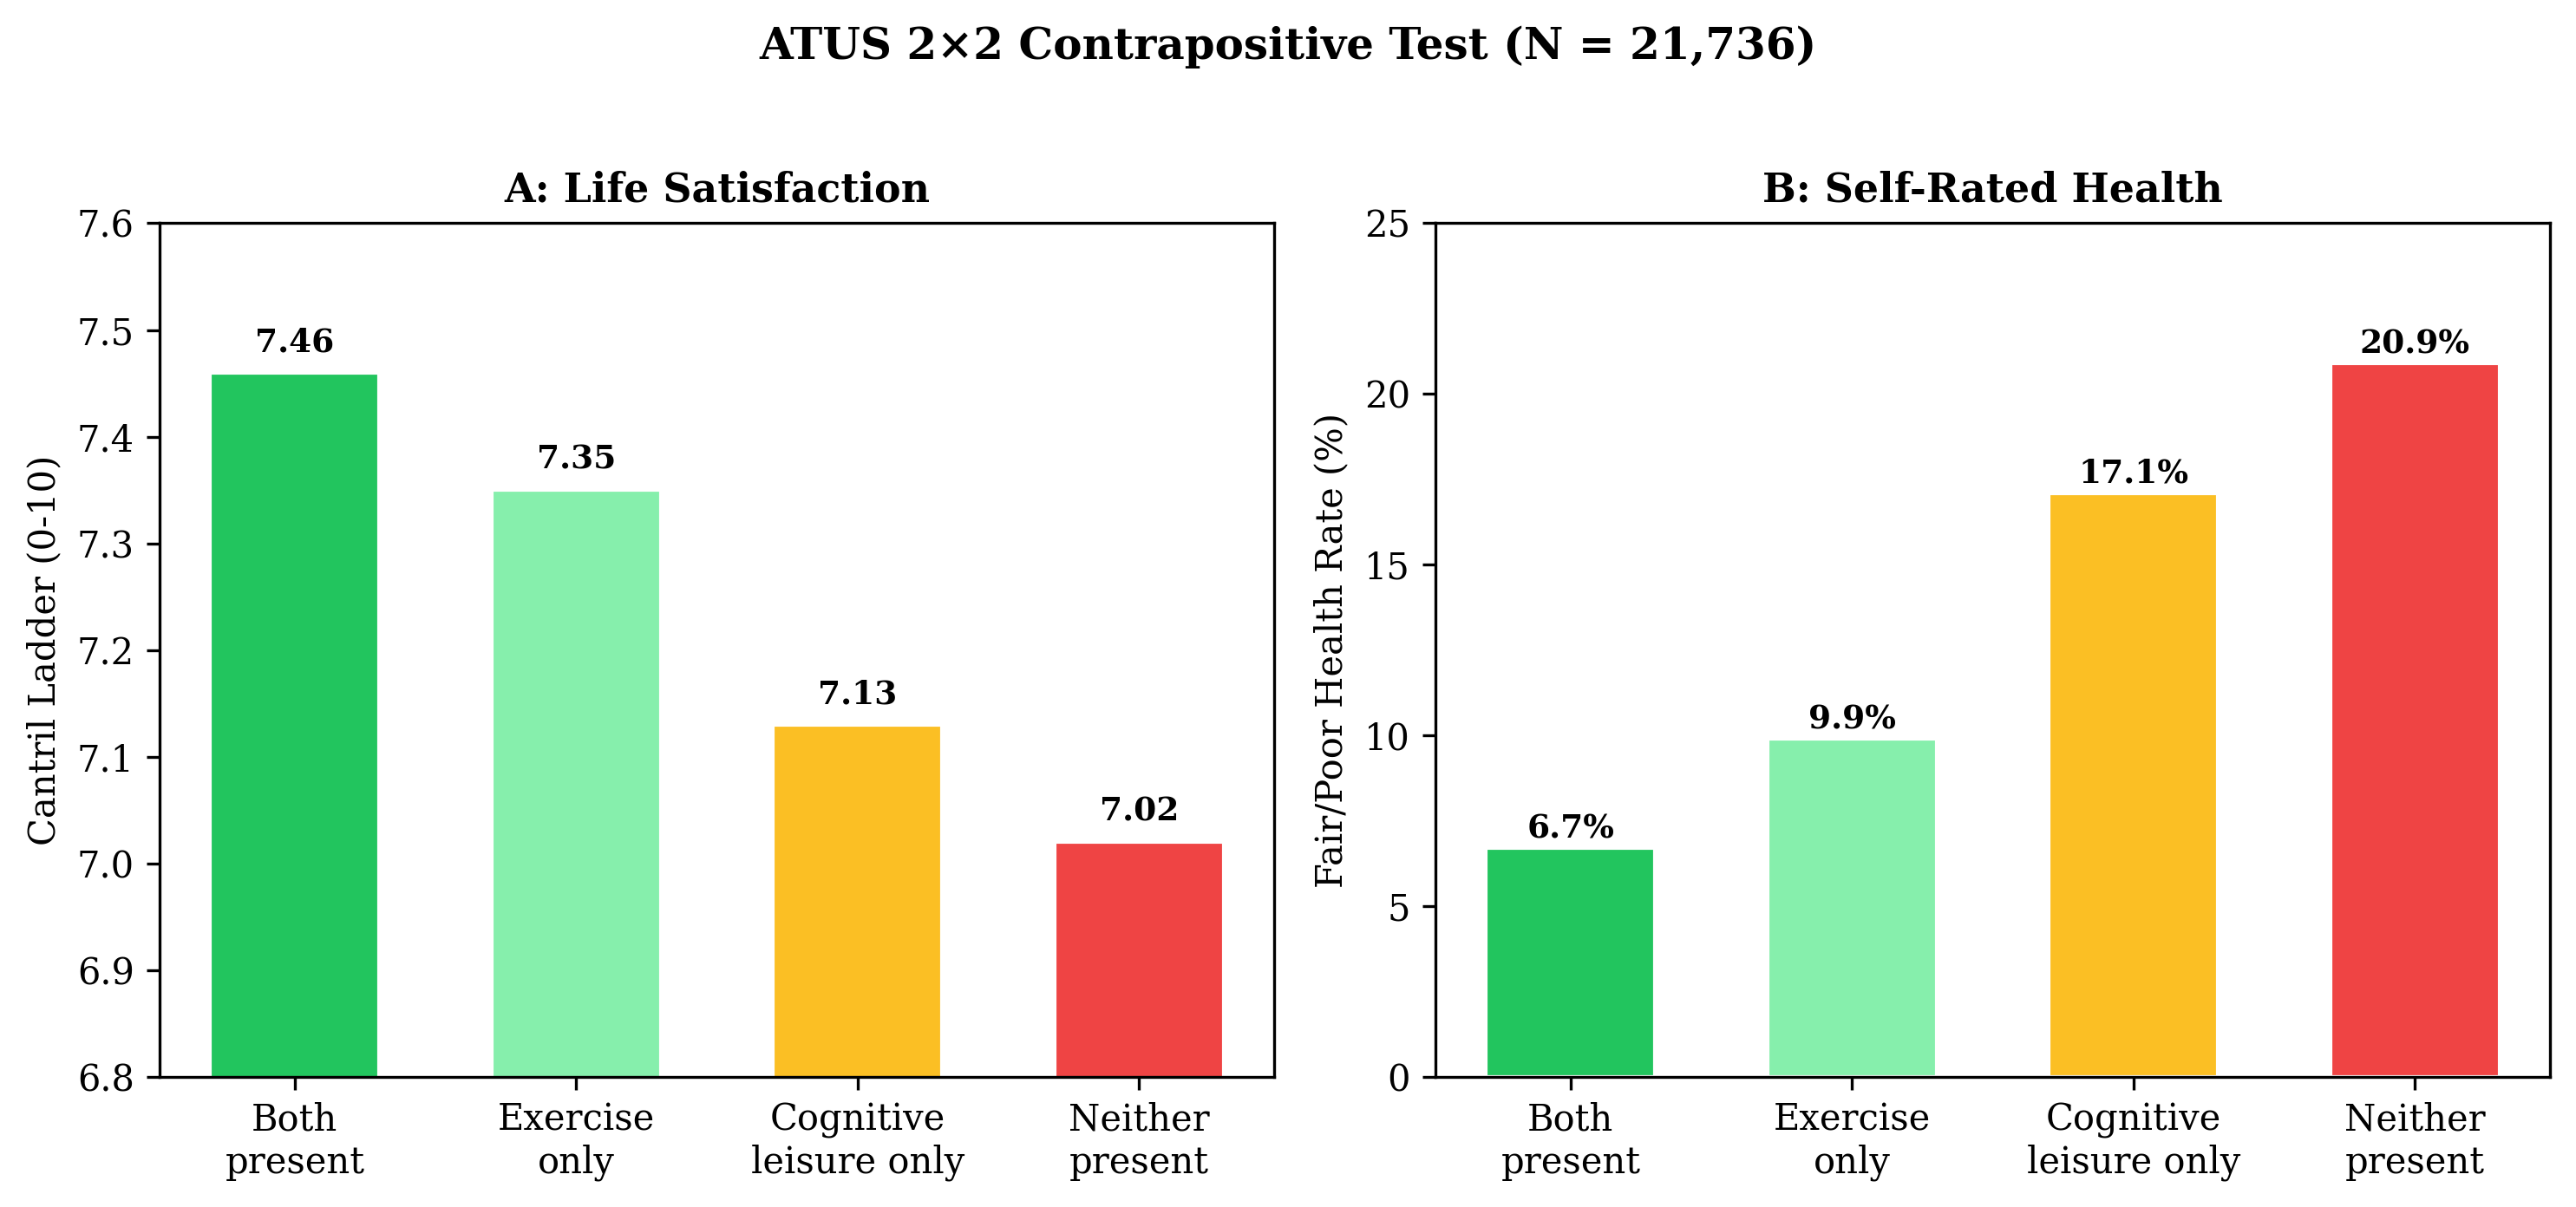
\includegraphics[width=0.95\textwidth]{fig04_atus_quadrant.png}
\caption{ATUS 2$\times$2対偶検証（$N = 21{,}736$）。A: Cantrilラダー（生活満足度）。B: Fair/Poor自己評価健康率。身体運動と能動的認知余暇の両方が不在の群は最悪の転帰を示す（Fair/Poor率3.1倍）。}
\label{fig:atus-quadrant}
\end{figure}

\begin{figure}[htbp]
\centering
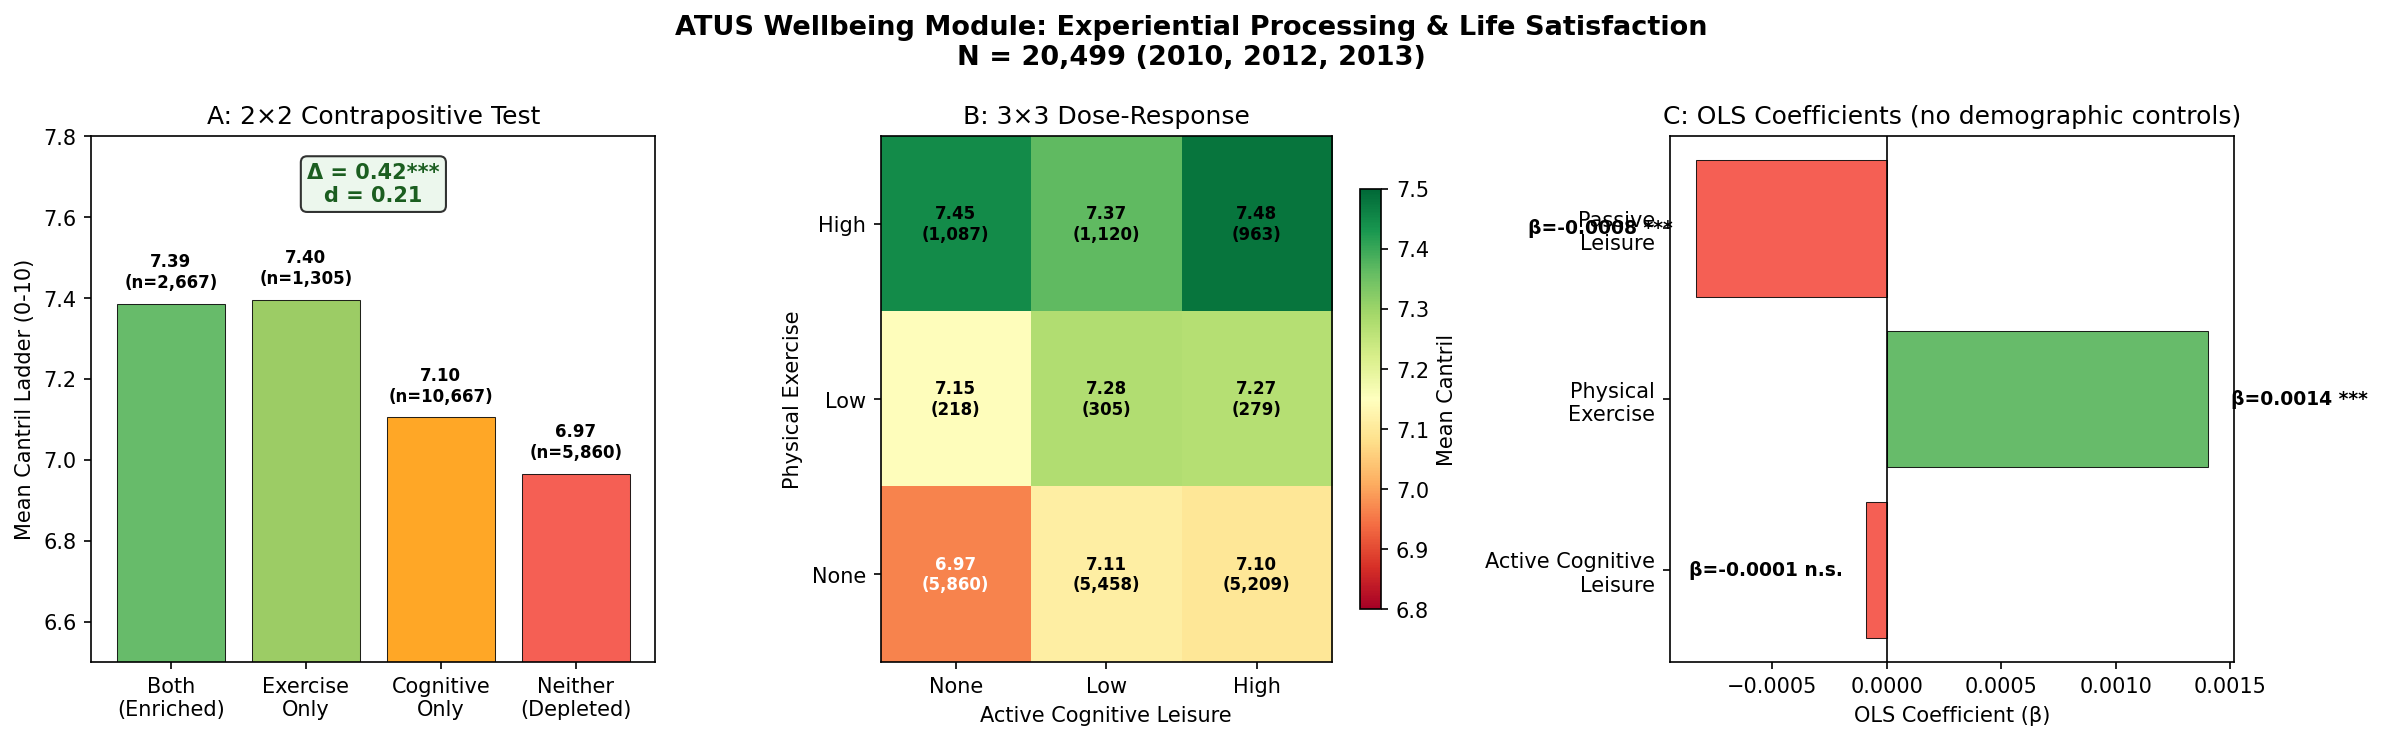
\includegraphics[width=\textwidth]{atus_wellbeing_analysis.png}
\caption{ATUS Wellbeing Module分析結果（$N = 21{,}736$）。A: 2$\times$2対偶検証（Cantrilラダー平均、$\Delta = 0.45^{***}$, $d = 0.23$）。B: 3$\times$3用量反応ヒートマップ。C: OLS係数（受動的余暇は負、身体運動は正の効果）。}
\label{fig:atus-data}
\end{figure}


\subsubsection{加法モデル vs 比率モデルの直接検証}\label{sec:ratio-test}

理論式$L = \alpha_1 I - \alpha_2 C$は加法構造を持つ。一方、マクロ分析では便宜的に比率proxy（Internet/Education）を使用した。ATUS個人データ（$N = 21{,}736$）を用いて、加法構造の妥当性を直接検証する。

5つの仕様を比較した（Table~\ref{tab:model-comparison}）。認知肥満比率$R = I/(C+1)$（受動的余暇分数/体験的処理分数）を構築し、加法モデル、比率モデル、対数比率モデル、2次対数比率モデル、バイナリ指標モデルのAIC・BICを比較した。

\begin{table}[htbp]
\centering
\caption{ATUS Wellbeing Module: 加法モデル vs 比率モデルの比較（$N = 21{,}736$）}
\label{tab:model-comparison}
\begin{tabular}{lccc}
\hline
モデル & AIC & $\Delta$AIC & $R^2$ \\
\hline
A: 加法（分単位） & \textbf{30,620} & 0 & 0.0108 \\
E: バイナリ指標（論文版） & 30,656 & +36 & 0.0091 \\
B: 比率 $R = I/C$ & 30,706 & +86 & 0.0066 \\
C: 対数比率 $\log(1+R)$ & 30,729 & +109 & 0.0056 \\
D: 2次対数比率 & 30,726 & +106 & 0.0058 \\
\hline
\end{tabular}
\end{table}

加法モデルがすべての仕様に対してAIC最良（$\Delta\text{AIC} \geq 36$）であり、理論式の加法構造を直接支持する。同時に、生の比率が測定誤差を増幅し分母の不安定性を生む問題に対し、成分別加法仕様の優位性を個人レベルで実証した。各成分の独立効果: 受動的余暇（$\beta = -0.0009$, $t = -11.08^{***}$）、身体運動（$\beta = +0.0016$, $t = 5.37^{***}$）。マクロ分析における比率proxyは国-年レベルの有用な近似であるが、個人レベルでは$\alpha_1 I$と$\alpha_2 C$が独立に作用することが確認された。

なお、比率$R$の五分位用量反応も方向性は一致する（Q1: Cantril $= 7.19$ → Q5: $6.93$, $d = 0.12$, $p < 10^{-7}$; Fair/Poor健康率: Q1 $= 13.8\%$ → Q5 $= 25.2\%$）。比率は理論の近似として有効だが、加法モデルの方が統計的に正確である（Figure~\ref{fig:ratio-test}）。

\begin{figure}[htbp]
\centering
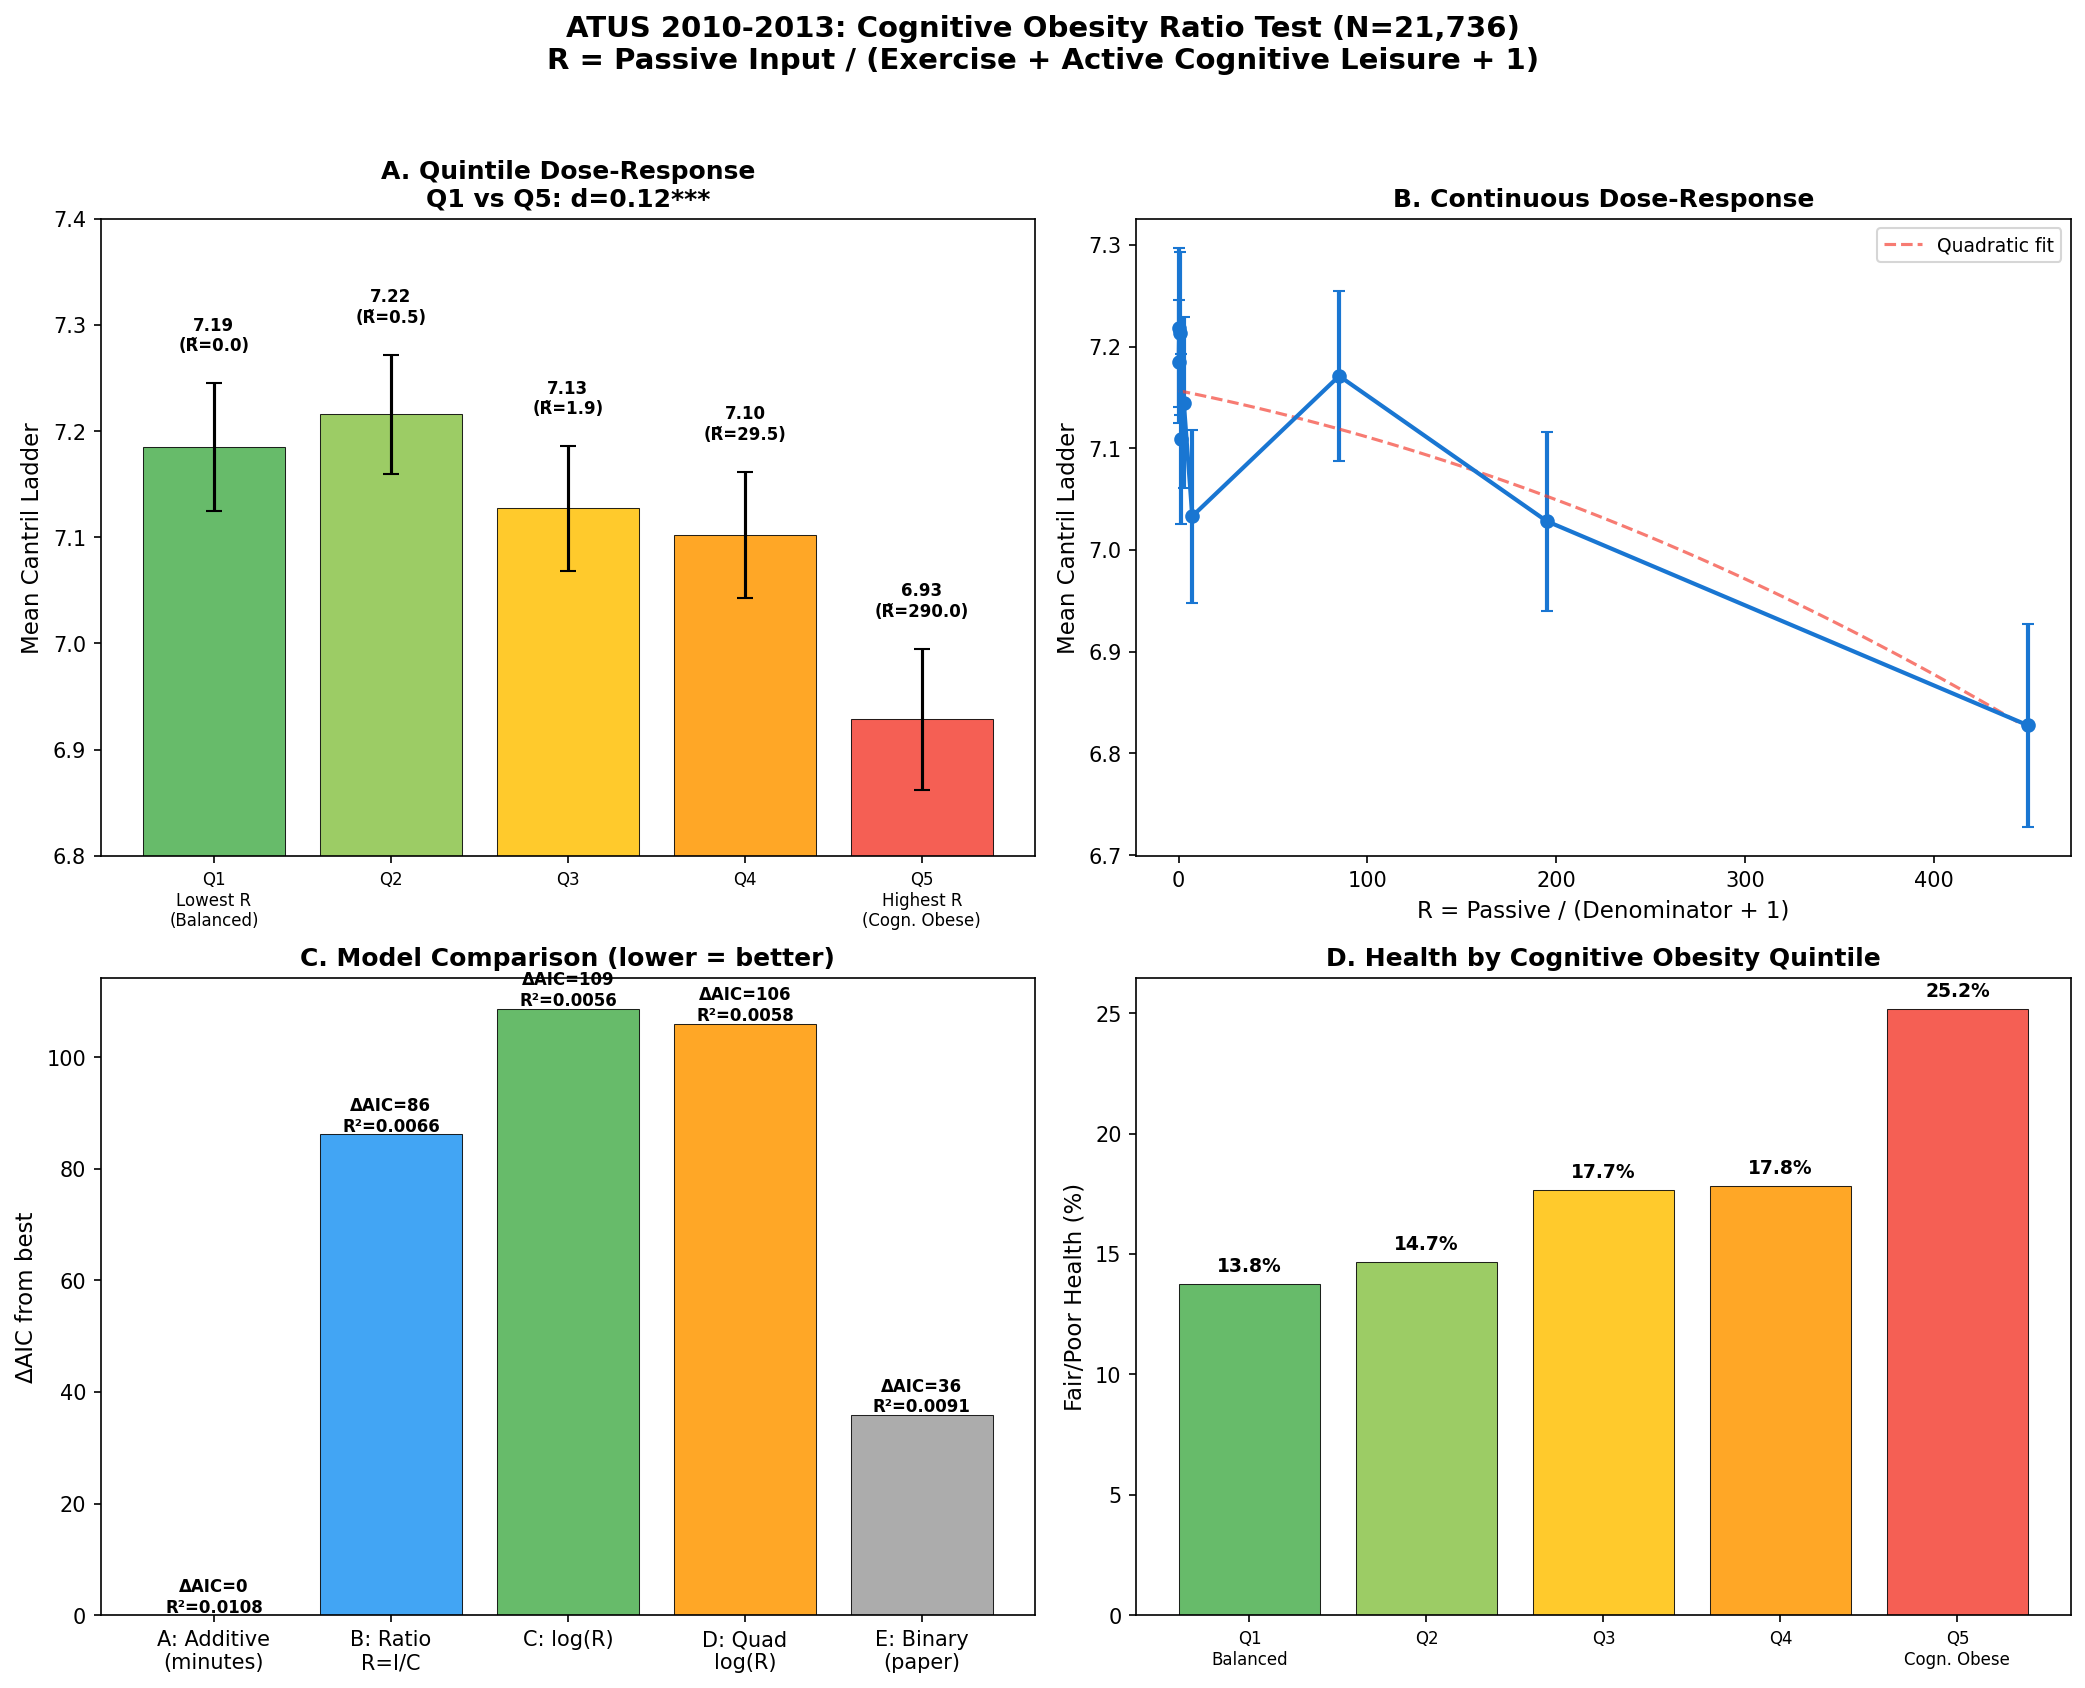
\includegraphics[width=\textwidth]{atus_ratio_test.png}
\caption{認知肥満比率の直接検証（$N = 21{,}736$）。A: $R$の五分位用量反応（Cantrilラダー）。B: 連続用量反応曲線。C: モデル比較（$\Delta$AIC; 加法モデルが最良）。D: 五分位別Fair/Poor健康率（Q1 $= 13.8\%$ → Q5 $= 25.2\%$）。}
\label{fig:ratio-test}
\end{figure}


\subsection{収束的証拠: 既存知見の再解釈}\label{sec:convergent}

以下は既存データの再解釈であり、バランスメカニズムの直接的因果検証ではない。バランスモデルが既存理論では生成できない新しい定量的予測を導出できることを示す。

\subsubsection{体験消費 vs 物質消費}

Van Boven \& Gilovich~(2003, JPSP)は「体験購買が物質購買より持続的に高い幸福度をもたらす」ことを示した。バランスモデルによる再解釈: 体験購買は第2項を直接増大させバランスを低下させ、物質購買は第1項（所有物の認知的管理）を慢性的に増大させる。Carter \& Gilovich~(2010)の知見---物質購買において選択しなかった代替案についての反芻が増大する---はこの再解釈を直接支持する。

\subsubsection{自然暴露の神経メカニズム（sgPFC-DMN）}

Bratman et al.~(2015, PNAS, $N=38$)は自然散歩でruminationとsgPFC血流が有意に低下することを示した。バランス的読み方: 自然環境は認知入力（第1項）が極小であり身体運動$+$感覚体験（第2項）が最大であるため、バランスを大幅に改善させる。都市散歩は身体運動は同等だが認知入力が高く、バランス改善が不十分である。

\subsubsection{認知的飢餓の処方的概念}

自然暴露の用量反応データ（Hunter et al. 2019; Bettmann et al. 2025, メタ分析78研究）: 最小有効量10分、天井効果は週200--300分。認知的肥満がバランスの慢性的上昇（第1項の過剰）であるならば、認知的飢餓はその意図的な逆転として定義できる。

\subsubsection{運動介入RCTエビデンス}

97のシステマティックレビューを統合したオーバービューレビュー（Singh et al. 2023, BJSM）: SMD $= -0.43$。Fernandez-Montero et al.~(2024): SMD $= -0.67$, NNT $= 2.78$。BMJネットワークメタ分析（Noetel et al. 2024）: 歩行、ジョギング、ヨガ、筋力トレーニングのいずれもが抗鬱薬と同等以上の効果量。

運動はバランスの第2項を直接的に増大させ、RCTでランダム化されている以上、この増大が鬱症状の改善を因果的に引き起こしている。

\subsubsection{自己効力感の再解釈}

Banduraの自己効力感は、本枠組みではループ閉合度の主観的評価として再解釈できる。Tak et al.~(2017)のクロスラグモデルが示す非対称的因果構造---鬱症状$\to$自己効力感低下（有意）だが逆方向は非有意---は、バランスモデルから自然に導かれる。


\subsection{差分的予測のまとめ: バランスモデル vs 既存理論}\label{sec:differential}

\begin{table}[htbp]
\centering
\caption{バランスモデルと既存理論の差分的予測}
\label{tab:differential}
\small
\begin{tabular}{p{3.5cm}p{3.5cm}p{3.5cm}p{3cm}}
\toprule
予測 & 検証条件 & ART/SRTの予測 & バランスモデルの予測 \\
\midrule
1. 自然$\times$スマホ交互作用 & 自然散歩中のスマホ併用 vs 非併用 & soft fascination存在 $\to$ 効果維持 & 第1項増大 $\to$ 効果減衰 \\
2. 屋内運動 vs 自然散歩 & 同等運動強度でのrumination比較 & コルチゾール同等なら同等効果 & 屋内$=$第2項のみ、自然$=$第1項低下$+$第2項増大 \\
3. 物質購買$\times$アレキシサイミア & 購買後rumination $\times$ TAS-20 & 予測なし & 高TAS-20$=$低い第2項 $\to$ バランス悪化大 \\
4. hedonic adaptation速度 & 購買後幸福度減衰速度 & 記憶価値で説明 & バランス変動量から定量予測可能 \\
\bottomrule
\end{tabular}
\end{table}

\cref{sec:macro,sec:individual}で提示した証拠は、マクロレベルの探索的分析と個人レベルの横断的・間接的証拠に基づく。バランスモデルの確認的検証には、個人内の時系列データによるリアルタイムのバランス変動と精神状態の関連の測定が不可欠である。\cref{sec:operationalization}では、この確認的検証に必要な操作化と研究デザインを提案する。


% ================================================================
% Section 5: Operationalization and Proposed Design
% ================================================================
\section{操作化と検証設計}\label{sec:operationalization}

\subsection{体験的処理の測定候補}

\begin{description}[leftmargin=2em]
\item[MAIA-2] Multidimensional Assessment of Interoceptive Awareness, Version~2（Mehling et al., 2018）。身体信号の気づきを8次元で測定。体験的処理容量の最も有望な個人レベル代理変数。
\item[TAS-20] Toronto Alexithymia Scale。慢性的な圧縮失敗を指標化する可能性がある。アレキシサイミア・鬱病・内受容感覚の三角形に注意。
\item[ESM] 経験サンプリング法。分単位の認知入力 vs 体験的処理バランスを捕捉。ウェアラブル統合により、スクリーンタイム$\times$身体活動のパターンをリアルタイムで追跡。
\end{description}

\subsection{提案ESMデザイン}

$n = 50$--$100$名、期間14日間、日8回プロンプト。ウェアラブル統合による自動身体活動検出。事前/事後測定: PHQ-9、TAS-20、MAIA-2。主要分析: 個人内バランスを時変動予測変数とするマルチレベルモデル。

検出力: Level~2 $= 50$名 $\times$ Level~1 $= 112$観測（日8回$\times$14日）の5,600観測で、80\%検出力が確保される（Arend \& Schäfer, 2019のシミュレーション指針に準拠）。

\subsection{最小コスト検証実験}

\paragraph{実験A（自然$\times$スマホ交互作用）.}
Bratman et al.~(2015)の追試に第3群「自然散歩$+$スマホ自由使用」を追加。$N = 60$（各群20名）。バランスモデルの予測: 自然散歩群のrumination低下$>$自然$+$スマホ群$>$都市散歩群。ARTの予測: 自然散歩群$\approx$自然$+$スマホ群$>$都市散歩群。fMRI不要のため実施コストはBratman et al.の$\approx 1/10$以下。

\paragraph{実験B（屋内運動 vs 自然散歩の分離）.}
$2 \times 2$被験者間デザイン: 運動条件（屋内トレッドミル vs 自然散歩）$\times$時間（事前 vs 事後）。各群25名。バランスモデルの予測: 自然散歩群のrumination低下$>$屋内運動群。

両実験合わせて参加者約110名、期間約3ヶ月、fMRI不要。学部レベルの卒業研究でも実行可能な範囲にある。


% ================================================================
% Section 6: Falsification Conditions
% ================================================================
\section{反証条件}\label{sec:falsification}

\subsection{反証条件6項目}

以下の結果が得られた場合、本枠組みの中核的主張は反証される:

\begin{enumerate}[label=\Roman*.]
  \item バランス変数（認知入力$-$体験的処理）が、個人レベルでスクリーンタイム絶対量を超える追加の分散を鬱病に対して説明しない。
  \item 感覚運動ループ閉合度を統制した後、ゲームとSNSが同等の鬱病リスクを示す。
  \item MAIA-2$\times$スクリーンタイム交互作用が鬱病に対してない（内受容感覚容量が緩衝しない）。
  \item インターネット/教育比が、マクロレベルでインターネット普及率単体よりも弱い鬱病予測因子である。
  \item 相関構造の相転移（高所得国 vs 低所得国）が、医療アクセスを統制すると消失する。
  \item 構造化された治療的AI（閉ループ設計）と汎用AI（自参照ループ許容）が、うつ症状への影響において同等の効果を示す（ループ構造が無関係）。
\end{enumerate}

\subsection{現時点の証拠の率直な評価}

\begin{table}[htbp]
\centering
\caption{現時点の証拠の評価}
\label{tab:honest}
\begin{tabular}{p{6.5cm}p{6.5cm}}
\toprule
本論文が提供するもの & 本論文が提供しないもの \\
\midrule
既存の混乱を再組織する新しい軸（バランス） & 個人レベルの確認的因果証拠 \\
予測と整合的なマクロレベル探索的証拠 & 高い説明力（$R^2 = 0.11$--$0.13$） \\
従来接続されなかった3つの文献の統合 & 「ループ閉合度」の直接的操作化 \\
具体的な反証条件 & 生態学的誤謬の解決 \\
検証ロードマップ & 個人レベルでバランス$>$絶対量の証明 \\
\bottomrule
\end{tabular}
\end{table}

マクロレベルの結果は探索的である。理論セクションは、個別には妥当で既存文献に接地しているが、その統合は新規であり未検証である複数の提案を含む。本枠組みは、確認済みの理論としてではなく、\textbf{検証可能な予測を生成する生産的な研究プログラムとして評価されるべきである}。

なお、NHANES（$d = 0.29$）とATUS（Fair/Poor健康率3.1倍）の個人レベル横断的証拠は「本論文が提供するもの」に追加されるが、因果方向は未確認であり、「提供しないもの」（確認的因果証拠）の制約は維持される。


% ================================================================
% Section 7: Discussion
% ================================================================
\section{議論}\label{sec:discussion}

\subsection{既存文献との位置づけ}

本枠組みは現在空白のニッチを占める。Haidt~(2024)とTwenge~(2017)は個人レベルのスクリーンタイム効果に焦点を当て、国際疫学やバランスベースのメカニズムを持たない。Achenbachの内在化/外在化分類は発展段階で層別化しない。置換仮説はバランスや処理モードを検討しない。

臨床心理学における行動活性化療法（BA）との関係は特に重要である。BAの「反芻$\to$直接体験への転換」は、本モデルの「自参照ループ$\to$閉ループへの転換」と同一の操作を異なる記述水準で表現したものである。BAの臨床的成功は、本モデルのバランスメカニズムの間接的な傍証として位置づけられる。

\subsection{政策的含意}

本枠組みが正しければ、現行の政策論争は構造的に不完全である。SNSの年齢制限とデジタルリテラシー教育はバランスの入力側のみを扱う。第2項---体験的処理容量---は全く異なる政策で扱われる: 体育の必修時間、屋外活動時間、芸術・工作のカリキュラム。

\textbf{核心的政策的洞察}: SNS年齢制限と体育の時間数は、代替案ではなく単一の政策パッケージとして扱われるべきである。

\paragraph{自然実験的示唆: 日本の働き方改革.}
日本の2018年働き方改革関連法は、強制的な残業上限規制による非選択的認知入力の政策的削減として解釈できる。日本の自殺率は2010--2017年（平均20.70）から2018--2021年（平均16.98）へ$\approx$17.9\%低下し、OECD比較8ヶ国の平均変化（$-0.2\%$）を大幅に上回った（DID推定値$= -17.7$パーセンテージポイント）。ただし、日本の自殺率は2003年のピーク以降一貫して低下トレンドにあり（pre-trend $= -0.39$/年）、働き方改革の効果と既存トレンドの分離は現在のデータでは困難である。因果的同定には改革の段階的適用を利用したより精密な分析が必要である。

\paragraph{倫理的留保.}
本枠組みは個人の情報アクセスを制限する根拠として用いられるべきではない。肥満研究の歴史が示すように、「太るのは自己責任」という個人帰責モデルは科学的にも倫理的にも破綻している。同様に、認知的肥満への対応は認知環境の再設計に向けられるべきである。権威主義的な情報統制の正当化に転用されるリスクには特に警戒が必要である。

\subsection{AI設計への含意: 認知運動化の原理}

本枠組みが正しければ、AIシステムは開ループや自参照ループを検知した際に、これを閉ループに変換する介入---「認知運動化」---を行うことで、認知的肥満を予防できる可能性がある。ループを切断するのではなく、同じエネルギーをより閉合度の高いループに転送する。

\paragraph{認知運動化の倫理的限界.}
重度うつ病患者に対してAIが行動変容を直接提案することのリスク、ループ検知の精度の問題、商業的AIにおけるsycophancyへの回帰インセンティブの問題がある。実装には安全策が不可欠である。

\subsection{観察問題}

同じ外的行動が、ある個人には認知入力を、別の個人には体験的処理を構成する可能性がある。プログラマーがコードをデバッグする場合は閉じた感覚運動ループを形成する。同じプラットフォームを受動的にスクロールするユーザーは開いたループを形成する。内受容感覚測定を伴うESMが、処理モードを直接指標化することでこれを解決する可能性がある。

\subsection{倫理的考慮}

サービス業構成の修飾効果は、認知的保護の不均等性という政策課題を浮き彫りにする。高所得層の正規雇用者には認知入力の時間的制限が制度化されているが、ギグワーカー、フリーランス、非正規雇用者にはこれらの保護が及ばない。認知的肥満対策は労働政策として設計される必要性が示唆される。

\subsection{「認知的飢餓」との関係}

認知的肥満が「入力 $\gg$ 処理」の状態であるならば、その鏡像として「認知的飢餓」（処理 $\gg$ 入力）も存在するはずである。候補となる状態には、知的刺激の乏しい環境（特定の施設、単調な労働）、感覚遮断、情報の乏しい環境が含まれる。このことから新しい予測が導かれる: 認知的飢餓と認知的肥満は異なる経路を経て類似の帰結（鬱、不安）に収斂するが、飢餓は退屈と刺激探索行動を伴い、肥満は圧倒感と回避行動を伴うはずである。この予測はESMで検証可能である。


% ================================================================
% Acknowledgments
% ================================================================
\section*{謝辞}
\addcontentsline{toc}{section}{謝辞}

本論文の筆者は情報理論・社会学・疫学のいずれにおいても専門的訓練を受けていない独立研究者である。本研究はAI（大規模言語モデル）との協働を通じて遂行された。直感的な仮説構築を筆者が、数値的検証・データ収集・統計分析・言語化をAIが担う形で進められている。この協働形態自体が、本論文が論じる「認知入力と体験的処理のバランス」という問題に対するひとつの実践的応答でもある。

本論文にはバイアスや検証前の直感的接続が残存している可能性が大いにある。探索的研究として仮説の問いかけのために公開するものであり、各分野の専門家による批判と検証を歓迎する。

全分析スクリプト、データ取得手順、および詳細な再現リポジトリは \url{https://github.com/miyauchikazuyoshi/cognitive-obesity-replication} で公開している。


% ================================================================
% References（簡略版 - 完全版はbibファイルで管理予定）
% ================================================================
\section*{主要参考文献}
\addcontentsline{toc}{section}{主要参考文献}

\begin{small}
\begin{enumerate}[label={[\arabic*]}, leftmargin=2em, itemsep=2pt]
  \item Barrett, L. F. (2017). \textit{How Emotions Are Made}. Houghton Mifflin Harcourt.
  \item Boers, E. et al. (2019). Association of screen time and depression in adolescence. \textit{JAMA Pediatrics}, 173(9), 853--859.
  \item Bratman, G. N. et al. (2015). Nature experience reduces rumination and subgenual prefrontal cortex activation. \textit{PNAS}, 112(28), 8567--8572.
  \item Carter, T. J. \& Gilovich, T. (2010). The relative relativity of material and experiential purchases. \textit{JPSP}, 98(1), 146--159.
  \item Chandra, K. et al. (2026). Sycophantic chatbots cause delusional spiraling. arXiv:2602.19141.
  \item Dimidjian, S. et al. (2006). Randomized trial of behavioral activation. \textit{JCCP}, 74(4), 658--670.
  \item Foley, P. (2025). AI, Cognitive Obesity and Arrested Development. \textit{Human-Centered Change and Innovation}.
  \item Granic, I. et al. (2014). The benefits of playing video games. \textit{American Psychologist}, 69(1), 66--78.
  \item Haidt, J. (2024). \textit{The Anxious Generation}. Penguin Press.
  \item Heinz, M. V. et al. (2025). Randomized trial of a generative AI chatbot for mental health treatment. \textit{NEJM AI}.
  \item Johannes, N. et al. (2021). Video game play is positively correlated with well-being. \textit{Royal Society Open Science}, 8(2).
  \item McBain, R. K. et al. (2025). Use of generative AI for mental health advice among US adolescents. \textit{JAMA Network Open}, 8(11).
  \item Mehling, W. E. et al. (2018). The Multidimensional Assessment of Interoceptive Awareness (MAIA). \textit{PLoS ONE}, 7(11).
  \item Noetel, M. et al. (2024). Effect of exercise for depression: systematic review and network meta-analysis. \textit{BMJ}, 384.
  \item Perlis, R. H. et al. (2026). Generative AI use and depressive symptoms among US adults. \textit{JAMA Network Open}, 9(1).
  \item Phang, J. et al. (2025). Measuring the impact of AI in the workplace. arXiv:2504.03888.
  \item Anthropic (2026). AI-powered disempowerment. arXiv:2601.19062.
  \item Pierre, J. M. et al. (2026). A case of new-onset AI-associated psychosis. PMC12863933.
  \item Roy, J. \& Orazem, P. F. (2021). Active and passive leisure. \textit{Economics of Education Review}.
  \item Singh, B. et al. (2023). Effectiveness of physical activity interventions for improving depression. \textit{BJSM}, 57(18), 1203--1209.
  \item Tak, Y. R. et al. (2017). The prospective associations between self-efficacy and depressive symptoms. \textit{J Youth Adolesc}, 46(10).
  \item Twenge, J. M. (2017). \textit{iGen}. Atria Books.
  \item Van Boven, L. \& Gilovich, T. (2003). To do or to have? \textit{JPSP}, 85(6), 1193--1202.
  \item Verduyn, P. et al. (2015). Passive Facebook usage undermines affective well-being. \textit{J Exp Psychol: General}, 144(2), 480--488.
  \item Watkins, E. \& Teasdale, J. D. (2001). Rumination and overgeneral memory in depression. \textit{J Abnorm Psychol}, 110(2), 353--357.
  \item Watkins, E. \& Teasdale, J. D. (2004). Adaptive and maladaptive self-focus in depression. \textit{J Affect Disord}, 82(1), 1--18.
  \item Whitworth, A. (2009). \textit{Information Obesity}. Chandos Publishing.
  \item Arend, M. G. \& Schäfer, T. (2019). Statistical power in two-level models. \textit{Psychological Methods}, 24(1), 1--19.
  \item Fernandez-Montero, A. et al. (2024). Physical activity and depression: umbrella review. 27 reviews, 190 trials.
  \item Mazzucchelli, T. G. et al. (2009). Behavioral activation treatments for depression. \textit{Clinical Psychology}, 16(4), 383--411.
  \item Orben, A., \& Przybylski, A. K. (2019). The association between adolescent well-being and digital technology use. \textit{Nature Human Behaviour}, 3(2), 173--182.
  \item Allcott, H. et al. (2020). The welfare effects of social media. \textit{American Economic Review}, 110(3), 629--676.
  \item Coyne, S. M. et al. (2020). Does time spent using social media impact mental health?: An eight year longitudinal study. \textit{Computers in Human Behavior}, 104, 106160.
  \item Hansen, A. (2019). \textit{Sk\"armhj\"arnan} [スマホ脳]. Bonnier Fakta.
  \item Csikszentmihalyi, M. (1990). \textit{Flow: The Psychology of Optimal Experience}. Harper \& Row.
  \item Nolen-Hoeksema, S. (1991). Responses to depression and their effects on the duration of depressive episodes. \textit{J Abnorm Psychol}, 100(4), 569--582.
  \item Ryan, R. M. \& Deci, E. L. (2000). Self-determination theory and the facilitation of intrinsic motivation. \textit{American Psychologist}, 55(1), 68--78.
  \item Varela, F. J., Thompson, E. \& Rosch, E. (1991). \textit{The Embodied Mind}. MIT Press.
  \item Caspi, A., et al. (2014). The $p$ factor: One general psychopathology factor in the structure of psychiatric disorders? \textit{Clinical Psychological Science}, 2(2), 119--137.
  \item Heffer, T., Good, M., Daly, O., MacDonell, E. \& Willoughby, T. (2019). The longitudinal association between social-media use and depressive symptoms among adolescents and young adults. \textit{Clinical Psychological Science}, 7(3), 462--470.
  \item Nickell, S. (1981). Biases in dynamic models with fixed effects. \textit{Econometrica}, 49(6), 1417--1426.
  \item Im, K. S., Pesaran, M. H. \& Shin, Y. (2003). Testing for unit roots in heterogeneous panels. \textit{Journal of Econometrics}, 115(1), 53--74.
\end{enumerate}
\end{small}


% ================================================================
% Appendix
% ================================================================
\appendix
\section{個人レベル分析の詳細仕様}\label{app:specs}

\subsection{NHANES 2017--2018分析仕様}

\textbf{データソース}: CDC NHANES 2017--2018サイクル。使用ファイル: DEMO\_J.XPT、DPQ\_J.XPT、PAQ\_J.XPT、BMX\_J.XPT、HIQ\_J.XPT。

\textbf{包含基準}: 20歳以上の成人、PHQ-9全9項目に有効回答、身体活動質問に有効回答。$N = 5{,}032$。

\textbf{モデル仕様}: (1)~2群比較（Welch $t$検定）。(2)~基本OLS: PHQ9 $= \beta_0 + \beta_1 \cdot \text{Exercise} + \beta_2 \cdot \text{Age} + \beta_3 \cdot \text{Sex} + \varepsilon$。(3)~フル共変量OLS（$+$Education, PIR, Insurance, BMI）。(4)~交互作用モデル（$+$SedentaryTime $+$ Exercise$\times$SedentaryTime）。全モデルで不均一分散に頑健な標準誤差（HC1）を使用。

\textbf{サーベイウェイトに関する注記}: NHANESサーベイウェイト（WTMEC2YR）は未適用。再現リポジトリにウェイト適用版を提供。

\subsection{ATUS Wellbeing Module 2010--2013分析仕様}

\textbf{データソース}: ATUS Wellbeing Module 2010--2013。$N = 21{,}736$。

\textbf{活動分類}: 受動的余暇（T120303$+$T120306）、能動的認知余暇（T120101, T1202xx, T120307--T120313, T1204xx）、身体運動（T1301xx）。

\textbf{分析手法}: 2$\times$2対偶検証、3$\times$3 dose-response、OLS回帰（交互作用の有意性検定）、フルバランステスト。

\textbf{限界}: 横断データ、サーベイウェイト未適用、共変量未投入、米国のみ。

\end{document}
